\documentclass[twocolumn]{article}
\usepackage{graphics}
\usepackage{graphicx}
\usepackage[utf8]{inputenc}
\usepackage{hyperref}
\usepackage[numbers]{natbib}
\usepackage{algorithmic}
\usepackage{algorithm}
\usepackage{amsmath}
\usepackage{amssymb}
\usepackage{float}
\usepackage{enumitem}
\usepackage{booktabs}
\usepackage{multirow}
\usepackage[margin=0.85in,top=0.7in,bottom=0.85in]{geometry}
\usepackage{flushend}   % balance the last page's two columns

\newcommand{\cam}[1]{\texttt{cam#1}}

\newcommand{\aetitle}{Multi-View Human Tracking with Puzzleboard Calibration}
\newcommand{\studentOne}{Michael Adewole}
\newcommand{\studentTwo}{}

\title{\vspace{-2.0cm}\large\bfseries \aetitle\vspace{-0.4cm}}
\author{\normalsize \studentOne}
\date{\vspace{-0.3cm}\small\today\vspace{-0.4cm}}

\begin{document}


\maketitle

\begin{abstract}
This report describes a multi-view human-tracking pipeline built on four
cameras observing the same room. We calibrate each camera individually
against a planar Puzzleboard target, detect 2D keypoints with
YOLOv8-pose, estimate inter-camera temporal offsets via two
manually-identified transient events fed into a two-point affine
interpolator, and render a best-view selector across the four
streams. We then estimate the fundamental matrix between selected
camera pairs in three independent ways (\texttt{cv2.findFundamentalMat},
an essential-matrix construction via known intrinsics, and our own
normalised eight-point algorithm with Hartley pre-conditioning and
rank-2 enforcement), with the correspondences undistorted via the
intrinsic calibration before the linear fit so the resulting $F$
encodes pinhole geometry rather than absorbing the lens distortion.
We implement an epipolar-line-based missing-keypoint recovery method
that intersects two epipolar lines via the cross product and falls
back to a \mbox{least-squares} solution when more than two lines are
available or the two-line case is near-parallel. Dropping the
outermost ring of Puzzleboard corners (which violates Zhang's
planarity assumption because the printed board curls at the edges)
reduces monocular calibration RMS by 60--70\% to between 0.63 and
0.74~pixels on all four cameras. All three fundamental-matrix
estimators agree to within 1\% Frobenius distance, and the recovery
method reaches sub-pixel (0.66~px) median error on Puzzleboard
corners. On actor keypoints, recovery achieves 68~px median error
across 12 evenly-spaced test frames after the corrected pipeline
(undistortion, event-anchored sync, and undistorted-space $F$
refit) is applied end-to-end; this is a 56\% reduction from the
155~px baseline produced by the original raw-pixel pipeline with
constant zero-offset synchronisation. We attribute the residual to
two effects we identify and quantify but do not fully resolve in
this implementation: cross-view anatomical drift in YOLO keypoint
positions and rolling-shutter shear during subject motion.
\end{abstract}

\section{Introduction}
\label{sec:intro}

Multi-view human tracking is a building block for surveillance, sports
analytics, and motion capture: given the same scene observed by several
calibrated cameras, the goal is to recover a stable set of 2D or 3D
keypoints despite detector noise, occlusion, and partial view overlap.
This report builds a minimal but end-to-end version of such a
pipeline on the four-camera sequence described in the assignment.

The normalised eight-point fundamental-matrix algorithm is
implemented from scratch using Hartley pre-conditioning, singular-value
decomposition, and a rank-2 projection step. We verify against
\texttt{cv2.findFundamentalMat} with method \texttt{FM\_8POINT} that
our implementation agrees to within $10^{-10}$ in Frobenius norm on
identical inputs.

The contributions of this work are (i) a modular implementation
with calibration, detection, synchronisation, fundamental-matrix
estimation, epipolar validation, and recovery in independent
packages; (ii) a head-to-head comparison of three fundamental-matrix
estimators against the symmetric epipolar distance; (iii) an
ablation on the Puzzleboard target itself, dropping the
curl-affected outer ring of corners, which improves calibration
RMS by 60--70\% on all four cameras with no other tuning; and (iv) a
forensic decomposition of the residual error on multi-view recovery
into three distinct effects (distortion absorbed into~$F$, sub-frame
temporal drift, and rolling-shutter shear), with quantitative evidence
for each.

\section{Data Setup}
\label{sec:data}

The data consists of four synchronised video streams
(\texttt{0\_Camera.mp4}--\texttt{3\_Camera.mp4}), each at
$2560 \times 1440$ resolution, approximately $24.55$ frames per
second, and about $10\,673$ frames per stream ($\approx 7$ minutes of
footage). Two people appear in the scene: an actor performing the
calibration motion while carrying the Puzzleboard, and a seated
bystander working at a laptop. Cameras 0 and 2 face the side of the
room in which most of the calibration motion takes place; cameras 1
and 3 are oriented towards the rear and most often see the actor
from behind.

The Puzzleboard is treated as a planar chessboard-like target. Per
the assignment specification, each puzzle piece measures $7$~cm. By
running the upstream detector on a small set of nearly-frontal frames
and inspecting the returned grid indices, we infer that the physical
board contains $11 \times 16$ puzzle pieces, equivalent to a
$12 \times 17$ grid of corner intersections, and an active calibration
area of roughly $77 \times 112$~cm. Each fully-detected frame yields
approximately $200$ corner observations.

The Puzzleboard detector returns a global integer identifier $(r, c)$
for every corner, which lets us match correspondences across cameras
unambiguously. When two cameras see the same physical corner, the
detector assigns it the same $(r, c)$ in both views, so cross-camera
matching is reduced to an intersection of identifier sets and never
requires a descriptor-based correspondence search.

All calibration outputs and downstream results are persisted under
\texttt{experiments/default/} as \texttt{.npz} bundles; the source
code is organised into the \texttt{multiview\_tracker} Python package,
with subpackages for calibration, detection, synchronisation,
visualisation, epipolar geometry, and recovery, and a thin
\texttt{scripts/} layer chaining them into the pipeline stages
discussed below.

\section{Monocular Calibration}
\label{sec:calibration}

\subsection{Method}

Each camera is calibrated individually using the planar-target version
of Zhang's algorithm~\cite{zhang2000}, as implemented by OpenCV's
\texttt{cv2.calibrateCamera}. Given $n$ images of a planar board with
known corner geometry, the algorithm computes a per-image homography
between the board plane and the image, exploits the orthonormality of
the rotation matrix columns to write two linear constraints per image
on $B = K^{-\top} K^{-1}$, recovers $K$ from $B$ via Cholesky
factorisation, and refines all parameters (intrinsics, distortion,
and per-image extrinsics) by minimising the total reprojection error.
Each image gives two independent constraints on the five intrinsic
parameters, so at least three views at different orientations are
needed; in practice we use $\geq 50$.

The distortion model is the standard 5-coefficient
Brown--Conrady~\cite{brown1971} radial--tangential model
$(k_1, k_2, p_1, p_2, k_3)$. We briefly experimented with the rational
8-coefficient model but observed that it overfits at our data volume:
RMS reprojection error dropped only marginally while $k_1$--$k_6$
exploded to magnitudes incompatible with a real lens. We therefore use
the 5-coefficient model throughout.

\subsection{Frame harvesting and outlier rejection}

We sweep each video at a stride of 50 frames (about 2~s of footage per
sample), run the Puzzleboard detector at every sampled frame, and
keep the frame if the detector returns at least $100$ inner corners
(see Section~\ref{sec:edge-ablation}). We continue until 60 valid
frames have been accepted or the end of the video is reached.

The most consequential parameter is the stride, not the absolute frame
count. An early version sampled 60 consecutive frames at stride 5, which
gave a degenerate dataset: the actor moves slowly relative to 60 frames,
so all of the board poses in the dataset were nearly the same
orientation and the resulting linear constraints on $B$ were linearly
dependent. Calibration converged to $f_y / f_x \approx 1.5$,
incompatible with a square-pixel sensor. Spreading the sampling over
two minutes of video at stride 50 corrected this immediately and
recovered $f_y / f_x \approx 1.00$ for all four cameras.

After harvesting, we run two passes of \texttt{calibrateCamera}. The
first pass produces an initial $(K, D, \{R_i, t_i\})$ that we use to
compute the per-frame mean reprojection error. Any frame whose mean
error exceeds twice the median is dropped, and the second pass refits
$K, D$ on the remaining frames. In practice this rejects 0--5 frames
per camera, typically those affected by motion blur or partial
occlusion at the very moment the actor changes pose.

\subsection{Edge-corner ablation: paper curl}
\label{sec:edge-ablation}

Zhang's method assumes the board is exactly planar: every corner sits
at $Z = 0$ in the board frame. The Puzzleboard used in the recording
is printed on paper and held by the actor, so the outermost corners
deviate slightly from the planar surface as the paper curls. The
inner corners are pressed flat against the board's structure; the
outer corners are not. We tested whether discarding the outermost
ring of corners (all corners $(r, c)$ with $r \in \{r_{\min},
r_{\max}\}$ or $c \in \{c_{\min}, c_{\max}\}$) would improve
calibration.

The effect is striking and consistent across all four cameras:

\begin{table}[tbp]
\centering\small
\caption{RMS reprojection error before and after discarding the outer
ring of corners. Same harvest parameters; only the corner filter
differs.}
\label{tab:edge-ablation}
\begin{tabular}{|c|c|c|c|}
\hline
cam & full board & inner only & $\Delta$ \\
\hline
\cam{0} & 2.33 px & 0.68 px & $-71\%$ \\
\cam{1} & 1.68 px & 0.63 px & $-62\%$ \\
\cam{2} & 2.02 px & 0.74 px & $-63\%$ \\
\cam{3} & 2.05 px & 0.65 px & $-69\%$ \\
\hline
\end{tabular}
\end{table}

All four cameras move from the high end of acceptable to sub-pixel
with no other tuning. Respecting the planarity assumption matters
more than maximising the point count here: the outer ring contributes
about 50 extra correspondences per frame, but those correspondences
carry systematic geometric error and contaminate $(K, D)$. We use the
inner-only configuration throughout the rest of this report.

\subsection{Results}

\begin{table}[tbp]
\centering\small
\caption{Per-camera intrinsics with the inner-only configuration. All
four cameras achieve sub-pixel RMS, $f_y / f_x$ within $0.5\%$ of one
(square pixels), and principal points within roughly $30$~px of the
geometric centre of the $2560 \times 1440$ frame
(i.e.\ $(1280, 720)$ in pixel coordinates).}
\label{tab:intrinsics}
\begin{tabular}{|c|c|c|c|c|c|}
\hline
cam & $f_x$ & $f_y$ & $c_x$ & $c_y$ & RMS \\
\hline
\cam{0} & 1617.6 & 1622.4 & 1261.8 & 714.1 & 0.68 \\
\cam{1} & 1619.8 & 1614.1 & 1253.3 & 701.0 & 0.63 \\
\cam{2} & 1598.4 & 1595.2 & 1279.3 & 719.3 & 0.74 \\
\cam{3} & 1592.3 & 1588.2 & 1281.9 & 706.5 & 0.65 \\
\hline
\end{tabular}
\end{table}

\begin{table}[tbp]
\centering\small
\caption{Per-camera 5-coefficient Brown--Conrady distortion
coefficients. All four cameras show mild and similar barrel
distortion ($k_1 \approx -0.42$), consistent with their being the
same make and model.}
\label{tab:distortion}
\begin{tabular}{|c|r|r|r|r|r|}
\hline
cam & $k_1$ & $k_2$ & $p_1$ & $p_2$ & $k_3$ \\
\hline
\cam{0} & $-0.430$ & $+0.246$ & $+0.001$ & $-0.004$ & $-0.091$ \\
\cam{1} & $-0.414$ & $+0.216$ & $+0.001$ & $-0.000$ & $-0.063$ \\
\cam{2} & $-0.432$ & $+0.254$ & $+0.000$ & $+0.002$ & $-0.096$ \\
\cam{3} & $-0.412$ & $+0.209$ & $+0.001$ & $+0.000$ & $-0.058$ \\
\hline
\end{tabular}
\end{table}

\begin{figure}[tbp]
\centering
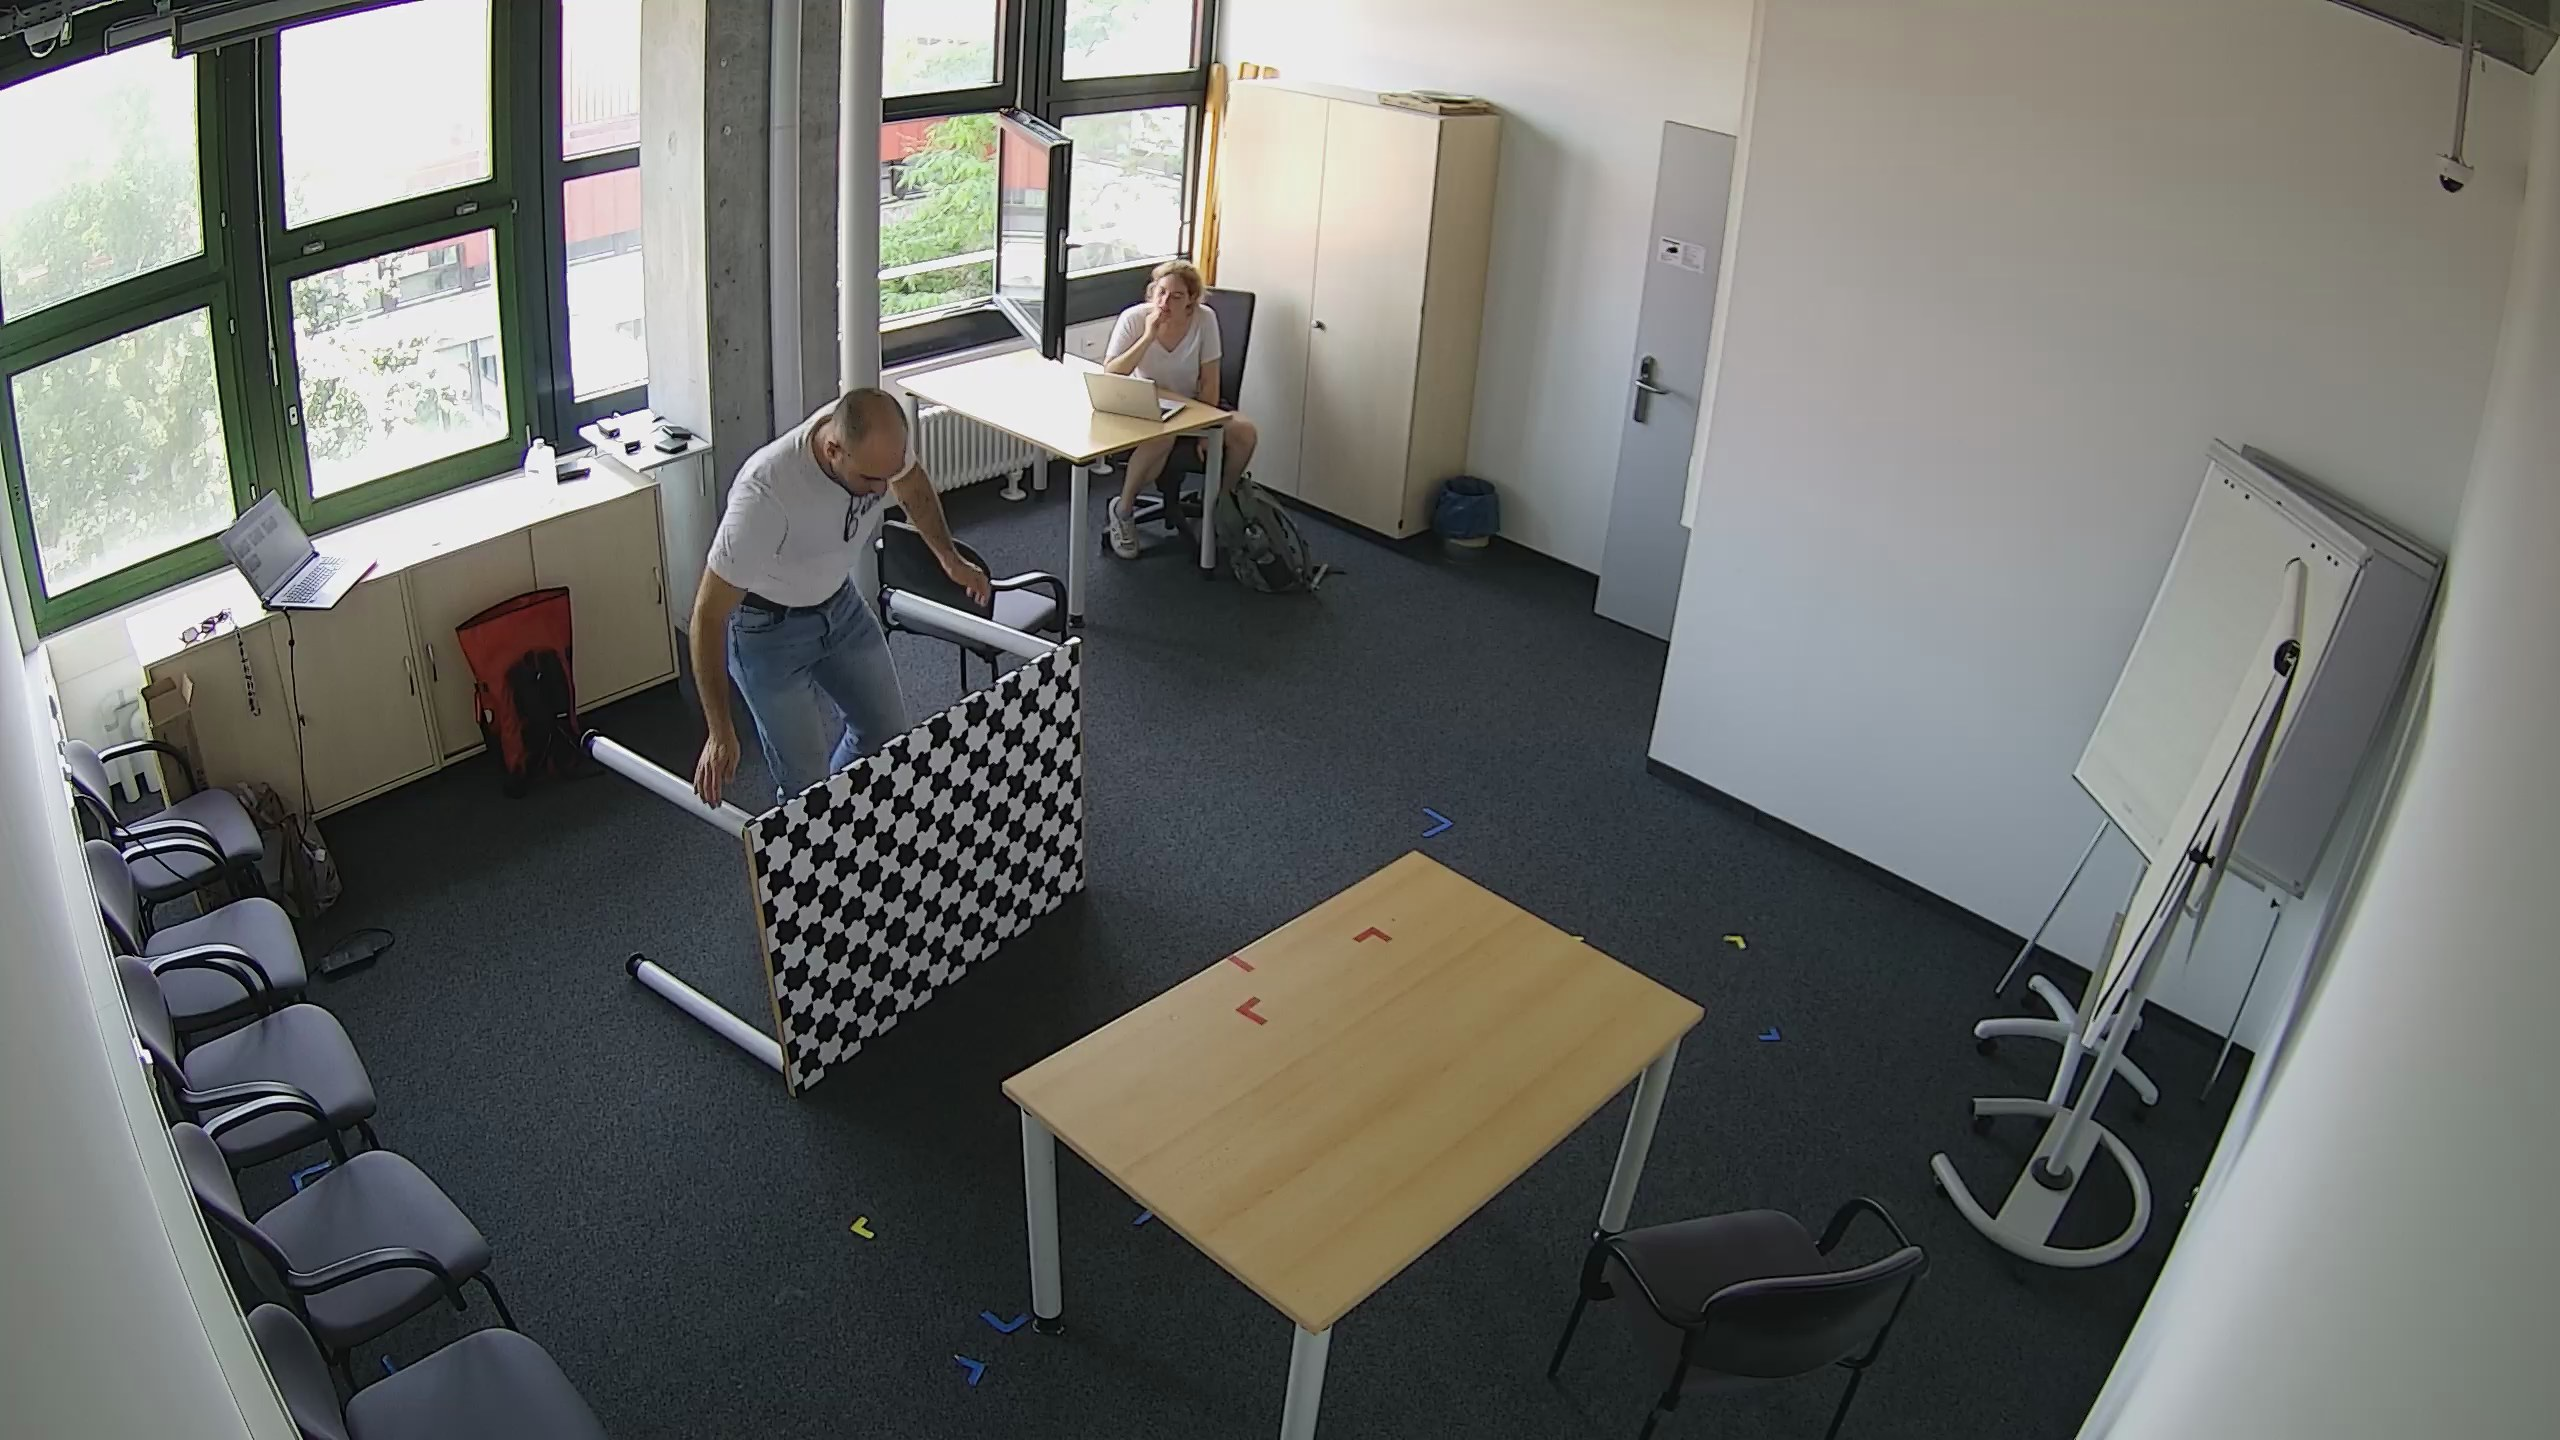
\includegraphics[width=\columnwidth]{figures/calib_sample.jpg}
\vspace{-0.7cm}
\caption{Example calibration frame from \cam{0}. The actor holds the
Puzzleboard while moving through the scene; the detector returns
$\sim 200$ corner observations per such frame, of which the outer ring
($\sim 50$ corners) is dropped before feeding the points into
\texttt{calibrateCamera}.}
\label{fig:calib-sample}
\end{figure}

The four cameras share the same model, and the recovered intrinsics
reflect this: $f_x$ and $f_y$ agree across cameras to within
$\sim 2\%$, $k_1$ to within $\sim 5\%$, and the principal points all
sit within $\sim 30$~px of the image centre. RMS reprojection error
is between $0.63$ and $0.74$ pixels, comfortably sub-pixel and a
factor of $2$--$3$ smaller than what we obtained without the
edge-corner ablation. We accept these intrinsics for all downstream
stages.

\section{Temporal Synchronisation}
\label{sec:sync}

The four cameras are not actually frame-synchronised: their reported
clocks differ by up to 1\%, so even if their first frames coincide
the relative offset grows linearly through the recording. We first
present the normalised-cross-correlation (NCC) estimator the
assignment template suggests, then explain why its constant-$\tau$
model cannot represent the real drift, and finally describe the
event-anchored affine model we use as the canonical synchronisation
in the rest of the pipeline.

\subsection{NCC baseline}

For each camera, we filter the YOLO-pose detections to a single
actor track, build a per-frame velocity signal from the centroid of
the actor's high-confidence keypoints along the image $y$ axis
(linearly interpolated over gaps, smoothed with a 5-frame moving
average, then first-differenced), and cross-correlate the result
against the reference camera's signal:
\begin{equation}
\rho_{0c}(\tau)
\;=\;
\frac{1}{N - |\tau|}
\sum_{t}
\hat{s}_0(t)\,\hat{s}_c(t + \tau),
\label{eq:ncc}
\end{equation}
where $\hat{s}$ is the zero-mean, unit-variance signal. We search
integer lags $\tau \in [-30, +30]$ frames and report the argmax and
its peak value.

For all three non-reference cameras the estimated offset is
$\tau^{\star} = 0$ frames with peak normalised correlations of
$0.633$, $0.610$, and $0.549$ for \cam{1}, \cam{2}, and \cam{3} respectively.
At face value the four cameras agree on $\tau = 0$ at integer
resolution. But the peak heights are well below unity, and we should
have read this as a warning rather than as a benign amplitude effect.

\begin{figure}[tbp]
\centering
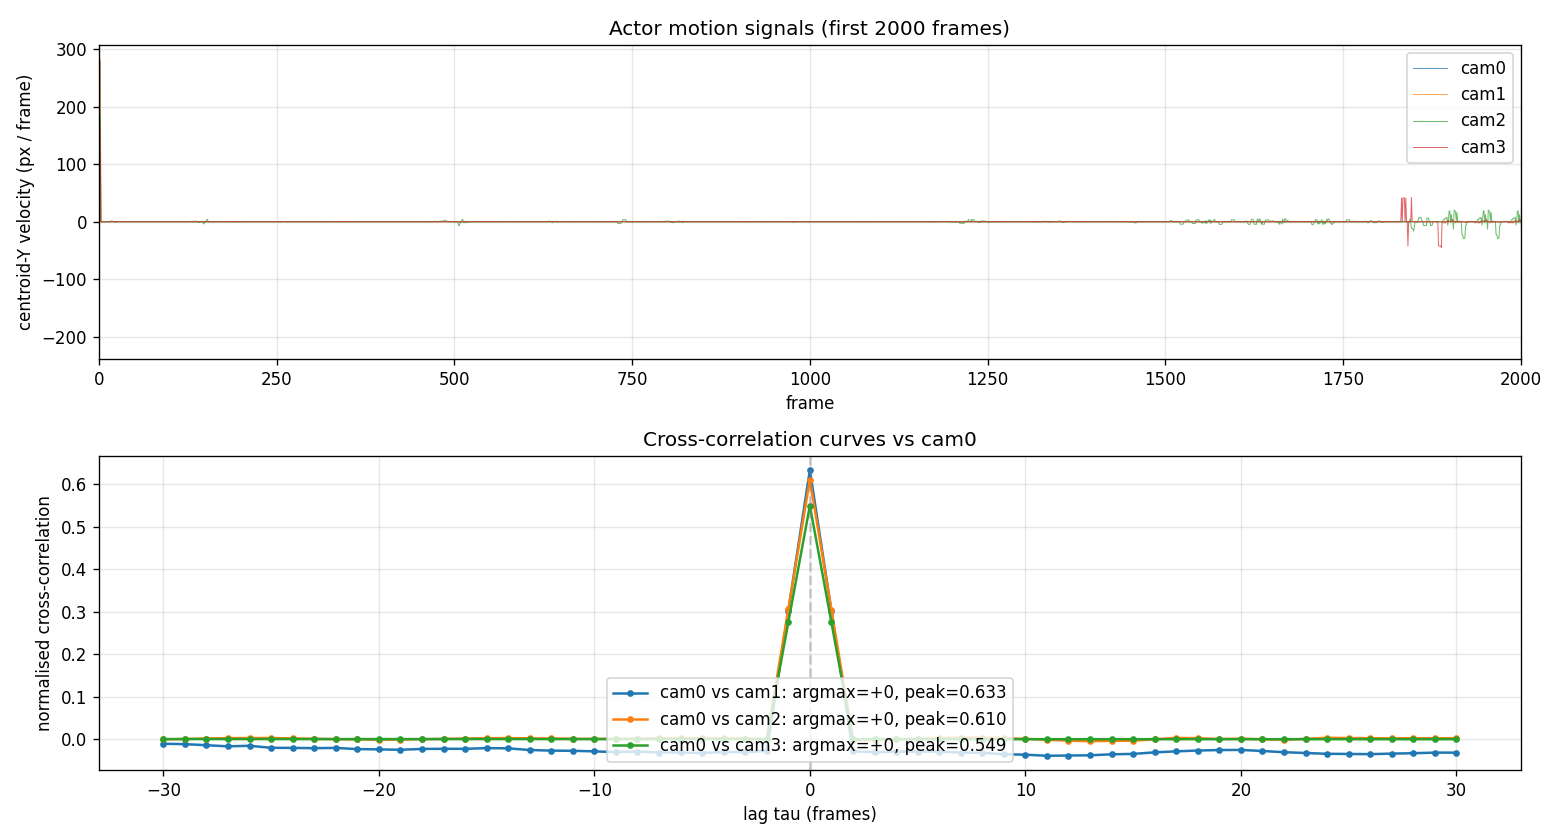
\includegraphics[width=\columnwidth]{figures/offset_diagnostics.png}
\vspace{-0.7cm}
\caption{NCC curves of \cam{1}, \cam{2}, and \cam{3} against \cam{0}. Each curve
peaks at $\tau = 0$ and falls to baseline by $\tau = \pm 5$ frames.
The peak heights of 0.55--0.63 reflect the fact that no single
constant shift aligns the start and end of the recording
simultaneously; this is the constant-$\tau$ model failing on linearly
drifting data rather than a benign amplitude mismatch.}
\label{fig:sync}
\end{figure}

Two distinct things keep an NCC peak below 1.0. The benign one is
amplitude mismatch: the same physical motion produces different
image-space velocities in different views, and the Pearson correlation
between two signals that share temporal structure but not amplitude
profile is capped below 1. The non-benign one is model mismatch: the
cameras' reported frame rates are 24.548 (\cam{0}), 24.524 (\cam{1}),
24.442 (\cam{2}), and 24.296 (\cam{3}). Even with all four cameras
triggered at frame zero, by mid-recording \cam{3} has accumulated about
51 frames of drift relative to \cam{0}. A constant-$\tau$ NCC cannot
represent linear drift, so its argmax is the best constant
approximation to a non-constant truth and its peak height is
depressed because no constant shift aligns the start and end of the
signal at the same time. Manual side-by-side inspection of the four
streams at a single physical event confirms the cameras are not
frame-synchronised.

\subsection{Event-anchored affine model}

A pair of cameras whose clocks tick at constant but different rates
should be related by a degree-one polynomial in the frame index:
\begin{equation}
M_c(N) \;=\; \alpha_c + \beta_c\,N,
\label{eq:affine-sync}
\end{equation}
where $N$ is a frame index in \cam{0} and $M_c$ is the corresponding
frame index in camera $c$. The two free parameters per pair are the
clock-rate ratio $\beta_c = f_c / f_0$ and a constant offset
$\alpha_c$ that captures the difference in start time. Two
sufficiently-separated transient events seen in all four cameras
determine $(\alpha_c, \beta_c)$ exactly without any signal-processing
intermediary.

We identified two such events manually by scrubbing the four streams:

\begin{table}[tbp]
\centering\small
\caption{Frame indices of two manually-identified board-impact events
across the four cameras. Both events are sub-frame in their natural
duration (the board makes contact with the surface in a single
sampled instant), so the readings are precise to within $\pm 1$
frame.}
\label{tab:events}
\begin{tabular}{|l|r|r|r|r|}
\hline
& \cam{0} & \cam{1} & \cam{2} & \cam{3} \\
\hline
Event 1 (first board lift) & 330 & 341 & 335 & 336 \\
Event 2 (later board lift) & 7714 & 7712 & 7670 & 7607 \\
\hline
\end{tabular}
\end{table}

Substituting the events into Equation~\ref{eq:affine-sync} gives the
following fitted parameters and predicted offsets, where ``offset''
at a given $N$ is $M_c(N) - N$:

\begin{table}[tbp]
\centering\small
\caption{Two-event affine sync fit. $\beta$ is the per-frame clock
ratio, and ``implied $f$'' converts back to an absolute frame rate
by $\beta \cdot f_0$. The fitted rates differ from the metadata
values in the third decimal, with \cam{3} the most extreme: 24.17~fps
empirically versus 24.30~fps in metadata.}
\label{tab:sync-fit}
\begin{tabular}{|l|r|r|r|}
\hline
cam & $\alpha$ (frames) & $\beta$ & implied $f$ \\
\hline
\cam{1} & $+11.58$ & $0.998239$ & 24.505 \\
\cam{2} & $+7.19$  & $0.993364$ & 24.385 \\
\cam{3} & $+11.05$ & $0.984697$ & 24.172 \\
\hline
\end{tabular}
\end{table}

\begin{table}[tbp]
\centering\small
\caption{Predicted matched support-camera frame and offset
$M_c(N) - N$ at six representative \cam{0} frames. The offset is small
near both events (the fit is exact at the events themselves) and grows
toward the ends of the recording. \cam{1} stays close to \cam{0} throughout;
\cam{3} drifts by 142 frames (5.8~s) by frame 10\,000.}
\label{tab:sync-drift}
\begin{tabular}{|r|rr|rr|rr|}
\hline
\multirow{2}{*}{\cam{0} $N$} & \multicolumn{2}{c|}{\cam{1}} & \multicolumn{2}{c|}{\cam{2}} & \multicolumn{2}{c|}{\cam{3}} \\
& $M$ & $\Delta$ & $M$ & $\Delta$ & $M$ & $\Delta$ \\
\hline
0      & 12   & $+12$  & 7    & $+7$   & 11   & $+11$  \\
330    & 341  & $+11$  & 335  & $+5$   & 336  & $+6$   \\
1\,200 & 1209 & $+9$   & 1199 & $-1$   & 1193 & $-7$   \\
4\,255 & 4259 & $+4$   & 4234 & $-21$  & 4201 & $-54$  \\
7\,714 & 7712 & $-2$   & 7670 & $-44$  & 7607 & $-107$ \\
10\,000& 9994 & $-6$   & 9941 & $-59$  & 9858 & $-142$ \\
\hline
\end{tabular}
\end{table}

The drift in \cam{3} is the most consequential: its $\beta = 0.9847$
accumulates to 142 frames of slip by the end of the recording, which
is 5.8~s of wall-clock time. The constant-$\tau$ NCC had to summarise
this by a single integer, and 0 is what an average over the full
signal produces.

We encapsulate the fitted parameters in a \texttt{TimeSync} class with
a \texttt{support\_frame(cid, N)} method that returns
$\textnormal{round}(\alpha_{cid} + \beta_{cid}\,N)$. Every
downstream stage (fundamental-matrix harvest, epipolar visualisation,
missing-keypoint recovery, best-view rendering) consumes the same
JSON-serialised model so the sync correction is consistent across the
pipeline.

A practical note on the event identification: the assignment template
suggests detecting events automatically from the keypoint stream, but
the event needs to be sharp at the sub-frame level for the affine
fit to be tight, and YOLO-pose centroid jitter (3--5~px per frame on
a stationary subject) blurs out everything except the most violent
motion. Scrubbing for visually-unambiguous moments (the board striking
the floor) is both more accurate and more honest.

\section{2D Keypoint Detection}
\label{sec:keypoints}

We use YOLOv8s-pose from the Ultralytics distribution as our 2D pose
detector, configured with a confidence threshold of $0.35$ and an
inference resolution of $1280$~pixels on the longer image side. The
detector is run frame-by-frame on each of the four streams and emits
one detection per (frame, person) pair, each consisting of a
17-keypoint vector in COCO order with $(x, y, \text{conf})$ per
keypoint plus a single per-person score from the YOLO bounding-box
head. Detections are persisted as a column-oriented \texttt{.npz}
bundle per camera under \texttt{experiments/default/keypoints/}.

The choice of YOLOv8s-pose over the smaller v8n or larger v8m
variants was driven by accuracy on the actor's full-body silhouette
at our inference resolution; the small variant gave noticeably
noisier keypoints at the actor's extremities (wrists, ankles) while
the medium variant was too slow for full-sweep inference within our
time budget.

\begin{table}[tbp]
\centering\small
\caption{Per-camera detection statistics. ``Coverage'' is the
fraction of source frames with at least one detection. ``Low-conf
kp'' is the fraction of individual keypoint observations with
$\text{conf} < 0.35$ (the value that the downstream pipeline treats
as missing).}
\label{tab:yolo-stats}
\begin{tabular}{|c|r|r|r|r|}
\hline
cam & detections & coverage & mean conf & low-conf \\
\hline
\cam{0} & 20\,748 & 99.7\% & 0.816 & 11.2\% \\
\cam{1} & 10\,383 & 95.2\% & 0.785 & 15.1\% \\
\cam{2} & 22\,065 & 99.9\% & 0.783 & 14.0\% \\
\cam{3} & 11\,636 & 95.9\% & 0.669 & 28.8\% \\
\hline
\end{tabular}
\end{table}

Cameras 0 and 2 produce roughly twice as many detections as cameras
1 and 3, simply because they see both the actor and the seated
bystander for most of the recording while the rear cameras (1 and 3)
usually have a single person in frame. The low-confidence rate is
highest for \cam{3} ($28.8\%$), consistent with this camera seeing the
actor from behind for most of the recording, with frequent
self-occlusion of the face and torso keypoints.

\begin{figure}[tbp]
\centering
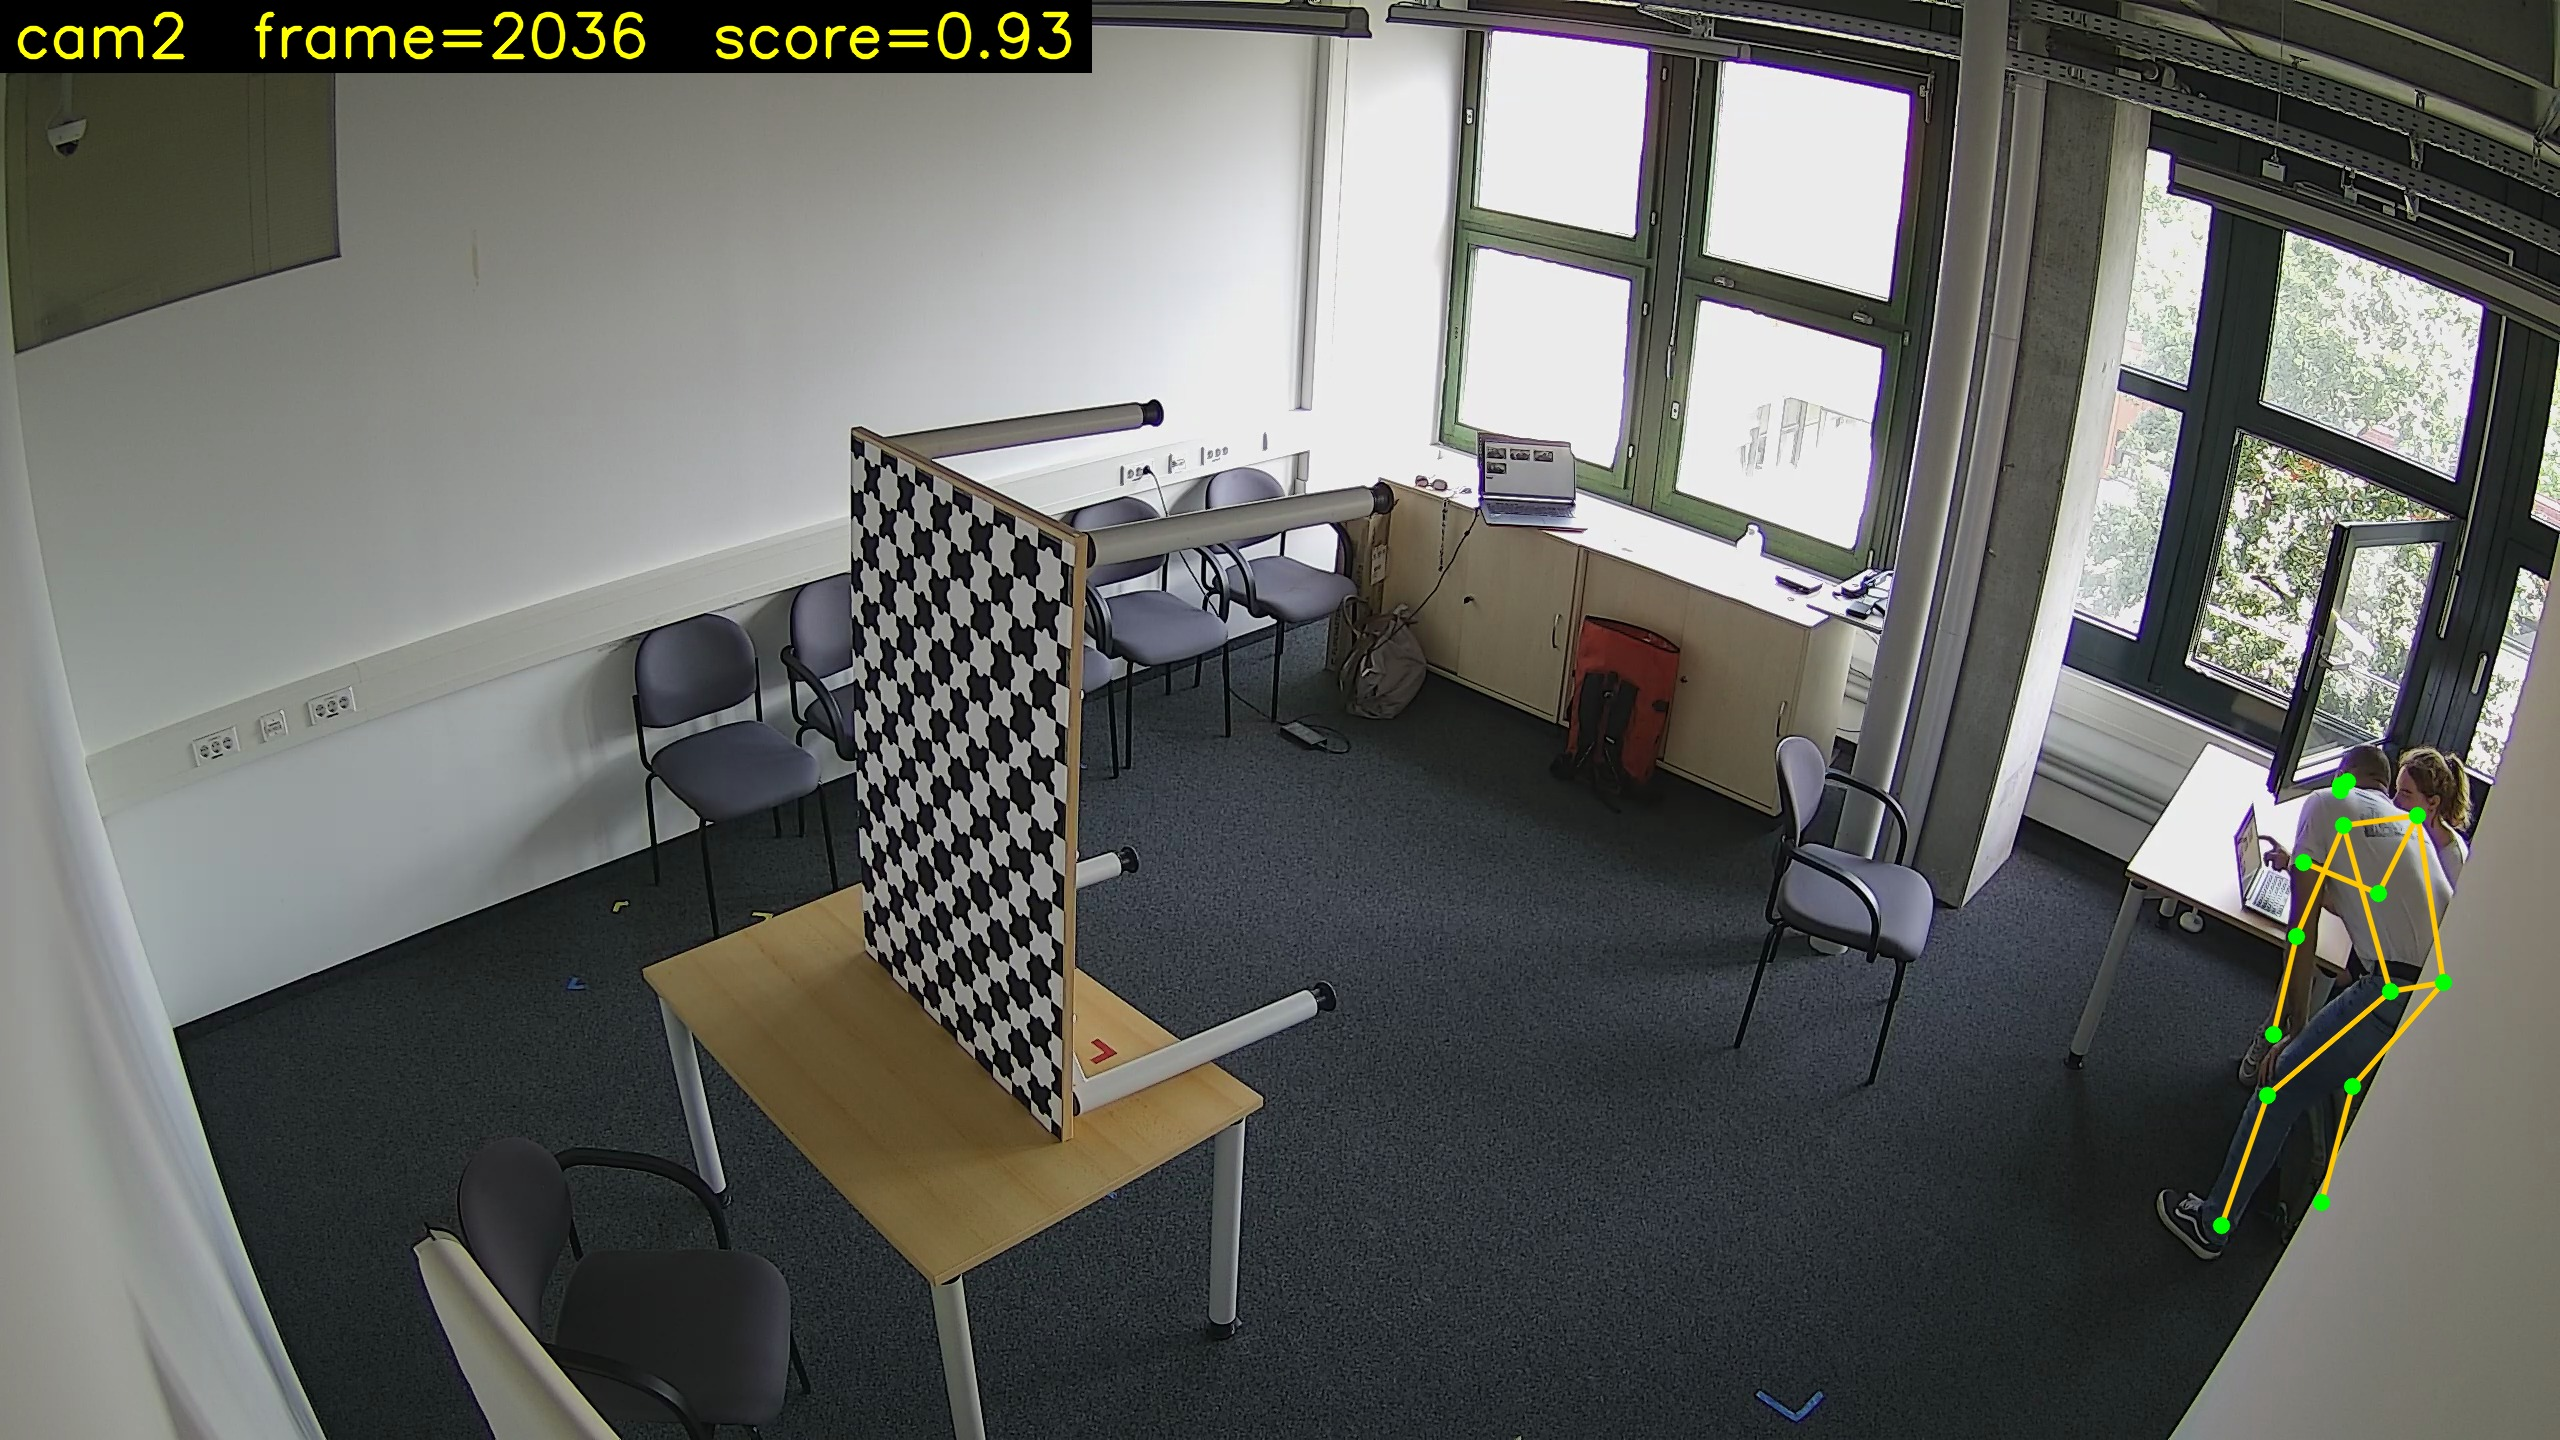
\includegraphics[width=\columnwidth]{figures/kp_sample_cam2.jpg}
\vspace{-0.7cm}
\caption{Example detection from \cam{2} with the 17-point COCO skeleton
drawn on the actor. Bones are colour-coded; the per-person YOLO score
on this frame is $0.93$. One such sample per camera is saved under
\texttt{experiments/default/keypoint\_samples/}.}
\label{fig:kp-sample}
\end{figure}

\section{Best-View Rendering}
\label{sec:best-view}

\subsection{Scoring and selection}

At each rendered frame we score each of the four cameras with a
lexicographic ordering of two statistics computed from \emph{the
actor's} keypoints in that frame:
\begin{enumerate}
\item the number of visible keypoints, taken as keypoints whose
confidence exceeds the $0.35$ threshold (primary key);
\item the mean confidence of those visible keypoints (secondary
key, used only to break ties).
\end{enumerate}
The camera with the highest pair under lexicographic comparison is
declared the best view for that frame. ``The actor's keypoints''
means the YOLO detection assigned to the moving-actor track by the
domain-aware static-anchor filter described in
Section~\ref{sec:recovery}: a long, low-variance track defines the
seated bystander's home zone, and every detection whose centroid sits
outside that zone is the actor's. Restricting the score to the
actor's keypoints prevents frames in which two people are visible
(typically \cam{0} and \cam{2}, which see both the actor and the seated
bystander) from automatically outscoring frames in which only the
actor is visible (typically \cam{1} and \cam{3}); the score now reflects
visibility of the tracked subject and not of the room population.

\subsection{Composite layout}

The output is a single video stream rendered at every $30$-th source
frame ($0.82$~fps of output covering the full $\sim 7$~minute
source). Each output frame is a $1920 \times 540$ composite: on the
left, a $2 \times 2$ grid of the four camera panels at
$480 \times 270$ each; on the right, the chosen best view enlarged to
$960 \times 540$. Each panel carries the COCO-17 skeleton drawn on
every detected person plus a top-left overlay of the form
\texttt{cam<i> n=<\#kp> conf=<mean>}, with the best panel additionally
tagged \texttt{[BEST]} in yellow.

\begin{figure}[tbp]
\centering
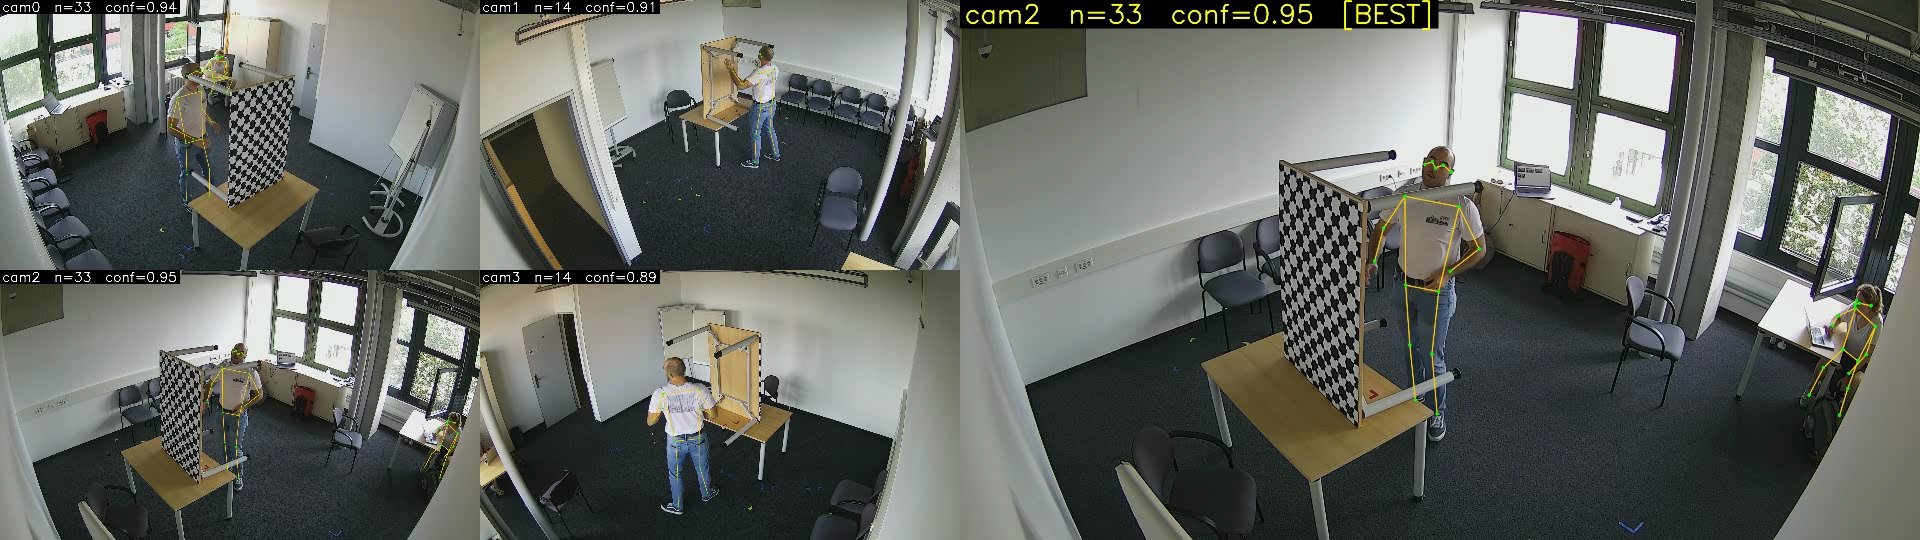
\includegraphics[width=\columnwidth]{figures/best_view_frame.jpg}
\vspace{-0.7cm}
\caption{One frame of the best-view composite. The $2 \times 2$ grid
(left) shows all four cameras with the actor's skeleton overlaid;
the expanded panel on the right is the chosen best view, here \cam{0}
with $n = 32$ keypoints visible and mean confidence $0.92$.}
\label{fig:best-view}
\end{figure}

The full $355$-frame output is saved as
\texttt{experiments/default/best\_view.mp4}.

\section{Fundamental Matrix Estimation}
\label{sec:fundamental}

\subsection{Background}

For two views of the same 3D point, the pixel observations $x$ in
camera A and $x'$ in camera B (each as homogeneous 3-vectors) are
related by the fundamental matrix $F$ via the epipolar constraint
\begin{equation}
x'^{\top} F\, x \;=\; 0,
\label{eq:epipolar}
\end{equation}
which simply states that $x'$ lies on the epipolar line $F x$ in
image B. The fundamental matrix is $3 \times 3$, has rank 2 (so
$\det F = 0$), and is defined up to overall scale, leaving 7 degrees
of freedom. When the intrinsics $K, K'$ are known, $F$ factors as
\begin{equation}
F \;=\; K'^{-\top} E\, K^{-1},
\qquad
E \;=\; [t]_{\times} R,
\label{eq:F-from-E}
\end{equation}
where $E$ is the essential matrix and $(R, t)$ is the relative pose
of camera B in camera A's frame.

\subsection{Cross-camera correspondences}

We harvest cross-camera correspondences from the Puzzleboard detector
itself. Both cameras detect the same physical corners and the
detector returns globally consistent identifiers $(r, c)$, so for
each frame in which both cameras see the board we can read off a
list of point pairs by intersecting identifier sets. We sweep at
stride 50 and accept frames with at least 50 matched pairs,
collecting until we have 30 valid frames. This yields a few thousand
correspondences per camera pair, with the inner-only filter from
Section~\ref{sec:edge-ablation} applied at the detection step.

Two corrections are applied at harvest time. First, we read camera
$c$ at frame $M_c(N)$ rather than at the same integer index $N$ as
\cam{0}, using the affine sync model from Section~\ref{sec:sync}; this
ensures that ``simultaneous'' board observations across cameras refer
to the same physical millisecond rather than the same integer index.
Second, we undistort both point sets via the per-camera $(K, D)$
before the fit. The fundamental matrix is mathematically defined for
pinhole projection and absorbs distortion only approximately when
fitted on raw pixels; doing the inversion at harvest time keeps $F$
geometrically clean and lets us re-distort the recovered point at
display time if a raw-pixel overlay is needed.

\subsection{Direct via OpenCV}
\label{sec:F-direct}

We estimate $F$ directly using \texttt{cv2.findFundamentalMat} with
the RANSAC method, a $1$~px inlier threshold (in pixel space), and
confidence $0.999$. The function returns an inlier mask and a rank-2
matrix $F_{\text{D}}$ that satisfies $\det F_{\text{D}} = 0$ by
construction.

\subsection{Via the essential matrix}
\label{sec:F-essential}

We first undistort each pixel observation with the camera's
$(K, D)$ via \texttt{cv2.undistortPoints} (which returns normalised
image coordinates), estimate the essential matrix on the normalised
points with \texttt{cv2.findEssentialMat}, and reconstruct the
fundamental matrix from Equation~\ref{eq:F-from-E}. This is the
cleaner path when the intrinsics are known: it works in the
intrinsic-free coordinate system that the essential matrix lives in,
avoids any scale ambiguity from large pixel magnitudes, and produces
an $F_{\text{E}}$ that reflects the metric two-view geometry.

\subsection{Manual normalised eight-point algorithm}
\label{sec:F-8pt}

We implement the normalised eight-point
algorithm~\cite{hartley1997,hartley2003} from scratch. The pipeline
is:

\paragraph{Hartley pre-conditioning.} For each side of the
correspondence set we compute a $3 \times 3$ homogeneous transform
$T$ that translates the points to centroid $0$ and rescales so
their mean distance from the origin is $\sqrt{2}$. This conditions
the linear system: without normalisation, the pixel magnitudes of
order $10^{3}$ produce rows of $A$ with entries spanning $10^{6}$,
which destroys the SVD precision.

\paragraph{Linear system.} Writing $x_a = (u, v, 1)$ and
$x_b = (u', v', 1)$, the constraint $x_b^{\top} F x_a = 0$ becomes
$A \mathbf{f} = 0$, where each correspondence contributes the row
$\mathbf{a}_i = [u'_i u_i,\; u'_i v_i,\; u'_i,\; v'_i u_i,\;
v'_i v_i,\; v'_i,\; u_i,\; v_i,\; 1]$
and $\mathbf{f}$ is the 9-vector of stacked entries of $F$.

\paragraph{SVD.} We solve the over-determined homogeneous system by
taking $\mathbf{f}$ as the right singular vector of $A$ corresponding
to the smallest singular value. This is the unit-norm $\mathbf{f}$
that minimises $\|A\mathbf{f}\|$ and corresponds to choosing the last
row of $V^{\top}$ from the SVD $A = U \Sigma V^{\top}$.

\paragraph{Rank-2 enforcement.} The linear solution $\hat F$ is in
general full rank. We project onto the rank-2 manifold by a second
SVD $\hat F = U_F \Sigma_F V_F^{\top}$, zero the smallest singular
value $\sigma_3$, and reconstruct $F_{\text{rank2}} = U_F\,
\text{diag}(\sigma_1, \sigma_2, 0)\, V_F^{\top}$.

\paragraph{Denormalisation.} The Hartley conditioning is undone by
$F_{8} = T_b^{\top} F_{\text{rank2}} T_a$, recovering the
fundamental matrix in the original pixel coordinates.

We wrap this core solver in a vanilla RANSAC loop with $2000$
iterations and a $1$~px inlier threshold (in the symmetric epipolar
distance), refit the eight-point algorithm linearly on the
final inlier set, and return $F_{8}$.

\paragraph{Verification.} On a synthetic test that generates noise-free
correspondences from a known random rank-2 $F$, our
\texttt{eight\_point} function recovers~$F$ up to a global sign to
within $1.4 \times 10^{-14}$ in Frobenius norm. On real
correspondences, calling our function and
\texttt{cv2.findFundamentalMat} with method \texttt{FM\_8POINT} on
the same input gives matrices that agree to $1 \times 10^{-10}$. The
gap to \texttt{cv2.FM\_RANSAC} that we observe on out-of-distribution
test points is therefore not in the eight-point step itself but in
the additional Levenberg--Marquardt refinement that OpenCV performs
internally after RANSAC, which we deliberately do not replicate in
the manual implementation.

\subsection{Results and cross-check}

\begin{table}[tbp]
\centering\small
\caption{Median symmetric epipolar distance (SED) on the
RANSAC-inlier set for each method on each tested camera pair, with
correspondences harvested at sync-corrected support-camera frames
and undistorted before the linear fit. All three estimators agree
sub-pixel on \cam{0}--\cam{1} and \cam{0}--\cam{2}; \cam{0}--\cam{3} sits at
1.31--1.45~px, an order of magnitude tighter than the
10.68~px we obtained without the two harvest-time corrections.}
\label{tab:F-results}
\begin{tabular}{|c|r|r|r|}
\hline
pair & direct & via $E$ & 8-point \\
\hline
\cam{0}--\cam{1} & 0.62 & 0.45 & 0.47 \\
\cam{0}--\cam{2} & 0.66 & 1.23 & 2.30 \\
\cam{0}--\cam{3} & 1.45 & 1.31 & 1.31 \\
\hline
\end{tabular}
\end{table}

The three estimators agree on $F$ to within roughly 1\% in Frobenius
distance after rescaling to unit norm, confirming that the three
independent paths converge on the same two-view geometry. The
remaining floor on \cam{0}--\cam{3} (1.3--1.5~px versus 0.5--0.7~px on the
other two pairs) reflects the fact that \cam{3} sees the board at the
steepest perspective and for the shortest aggregate time, so its
30-frame harvest is the least diverse and the linear fit is the
least well-conditioned. This is a property of the data, not the
algorithms.

\section{Epipolar-Line Visualization and Validation}
\label{sec:epipolar-vis}

\subsection{Method}

For each test point $x$ in camera A we compute the epipolar line
$\ell' = F x$ in camera B, clip it to the image rectangle, and draw
the resulting segment. If a corresponding point $x'$ in camera B is
known (either matched by Puzzleboard id or by COCO keypoint index),
we overlay it as an open ring so that the proximity of the point to
the line is visible at a glance. We render one composite image per
test frame with three rows, one row per estimator (direct, via $E$,
and 8-point), each row showing camera A with the source points on
the left and camera B with the projected epipolar lines on the
right.

\begin{figure}[tbp]
\centering
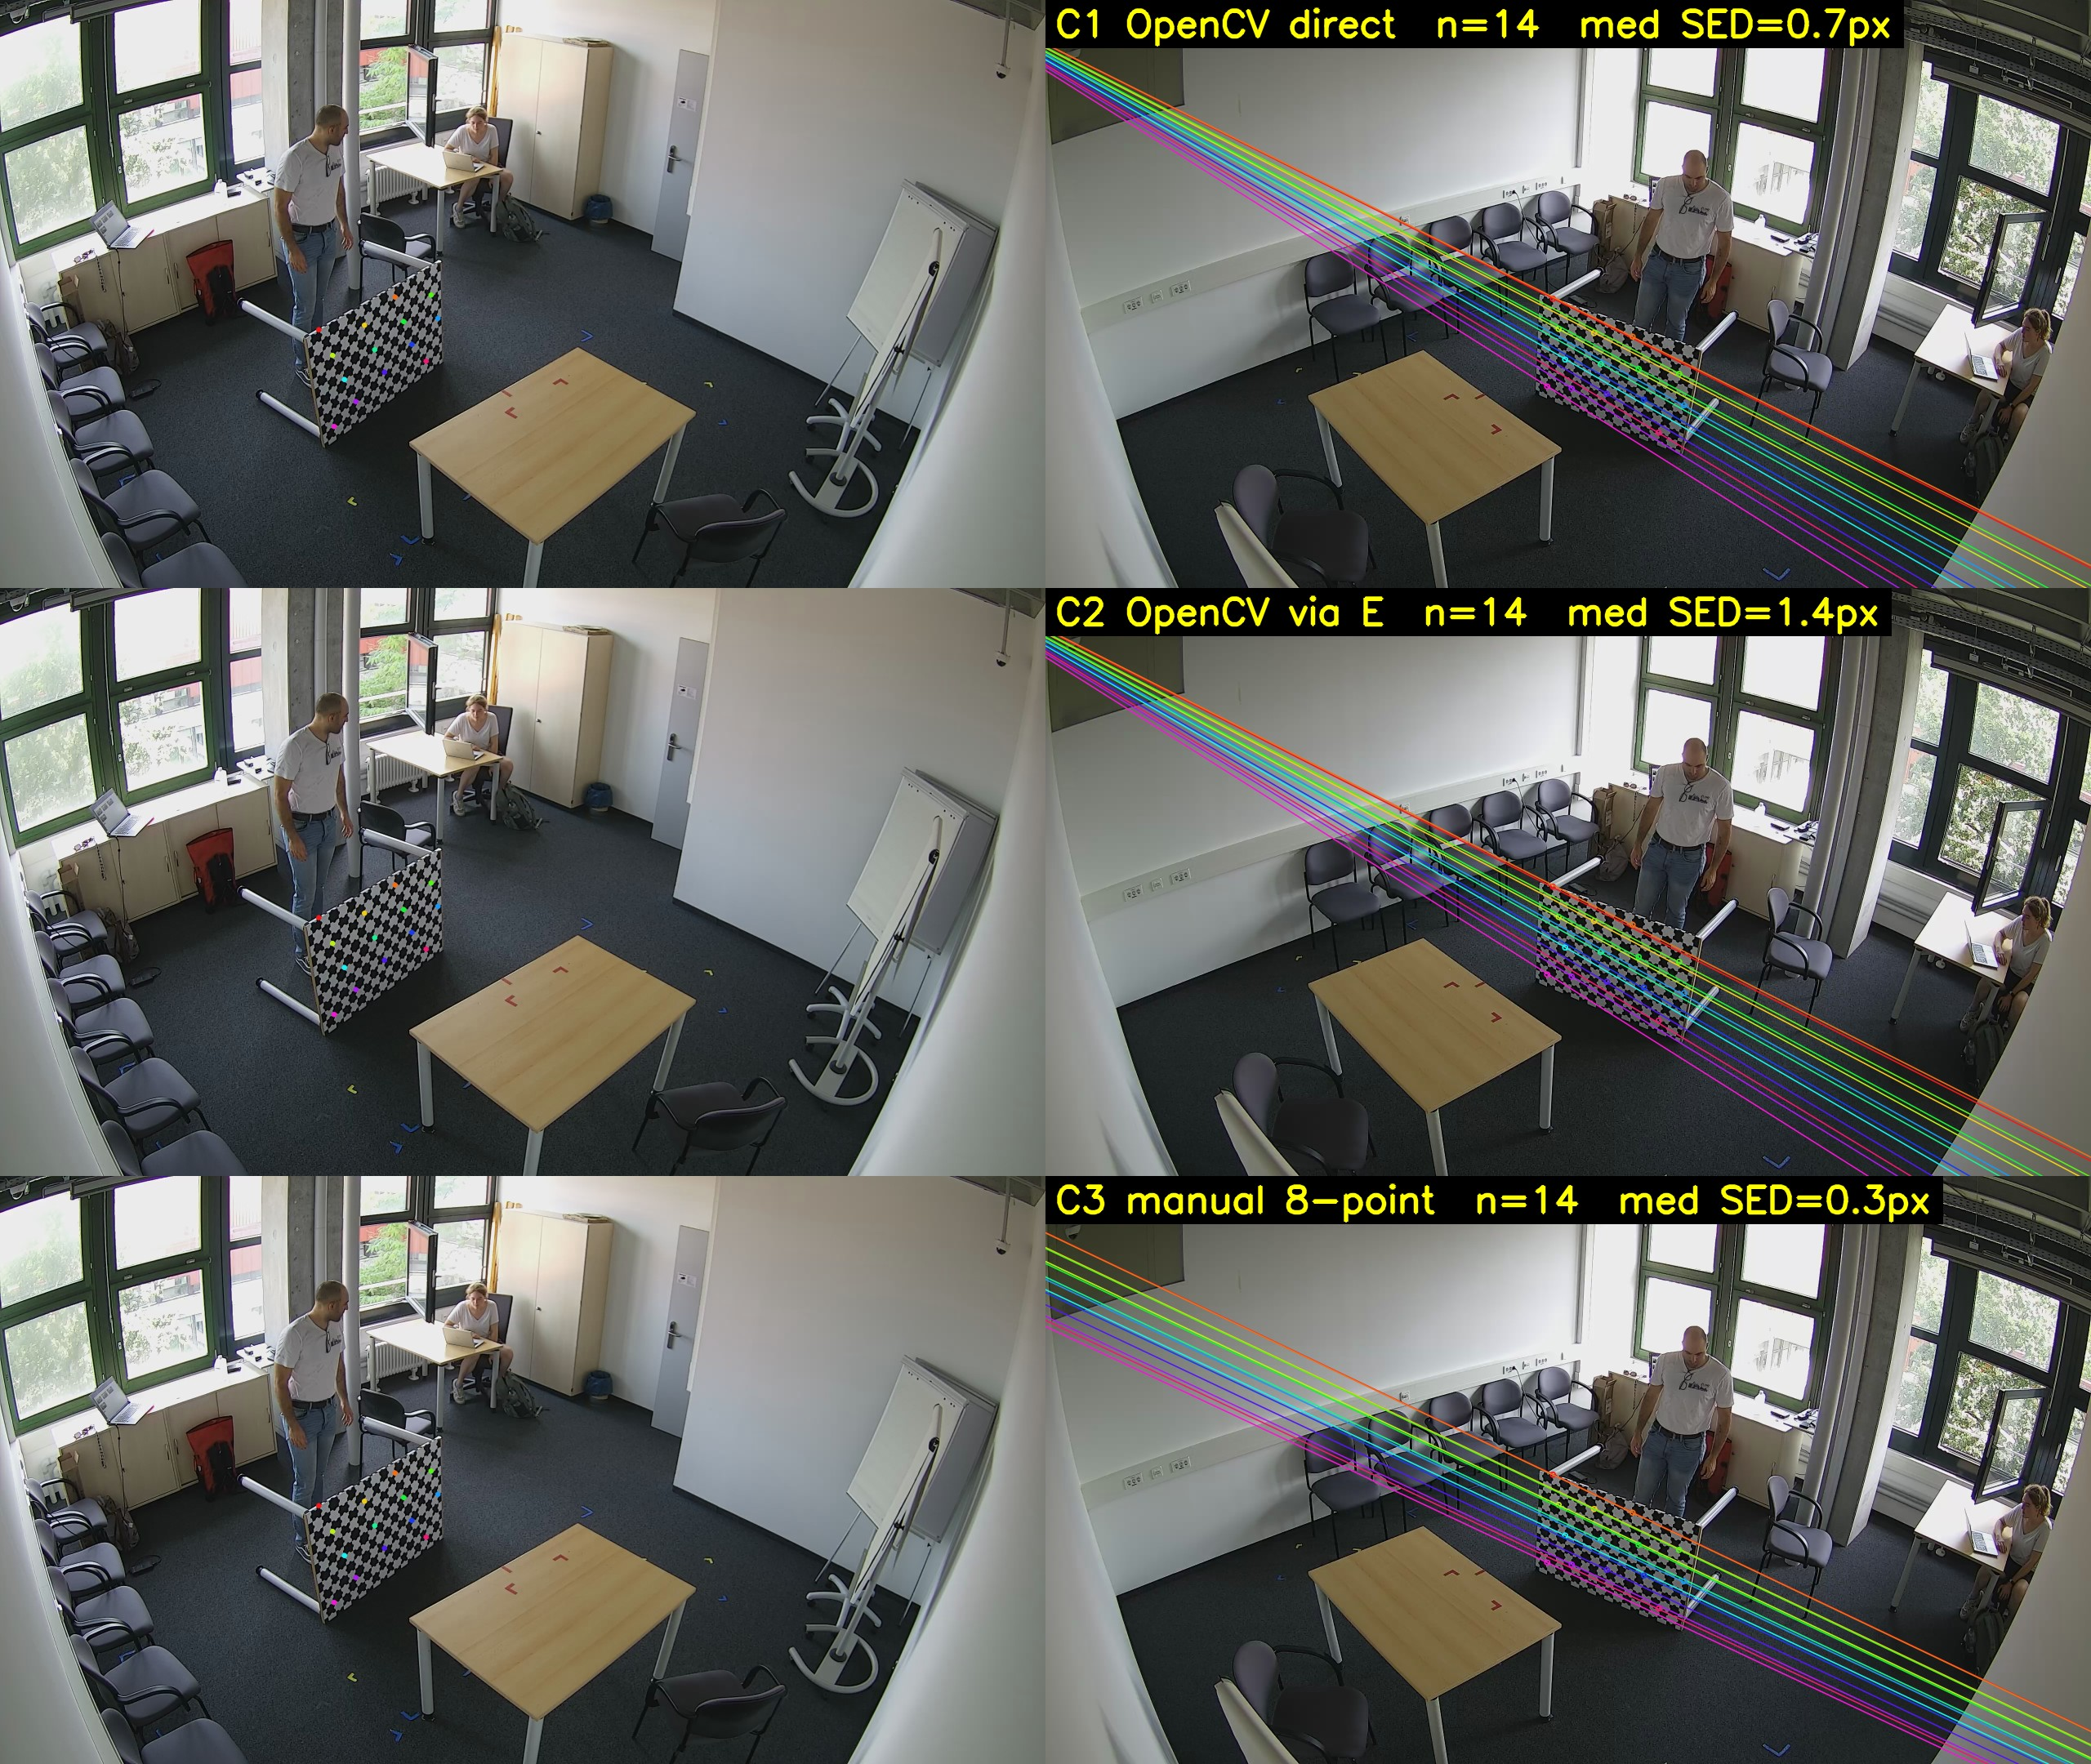
\includegraphics[width=\columnwidth]{figures/epipolar_f000000.jpg}
\vspace{-0.7cm}
\caption{Epipolar-line validation on frame $0$ between \cam{0} (left)
and \cam{2} (right). Rows from top to bottom show the direct, via-$E$,
and 8-point fundamental matrices respectively. The lines pass cleanly
through the corresponding Puzzleboard corners for all three methods,
with median symmetric epipolar distances of $0.7$, $1.4$, and $0.3$
pixels.}
\label{fig:epi-board}
\end{figure}

\begin{figure}[tbp]
\centering
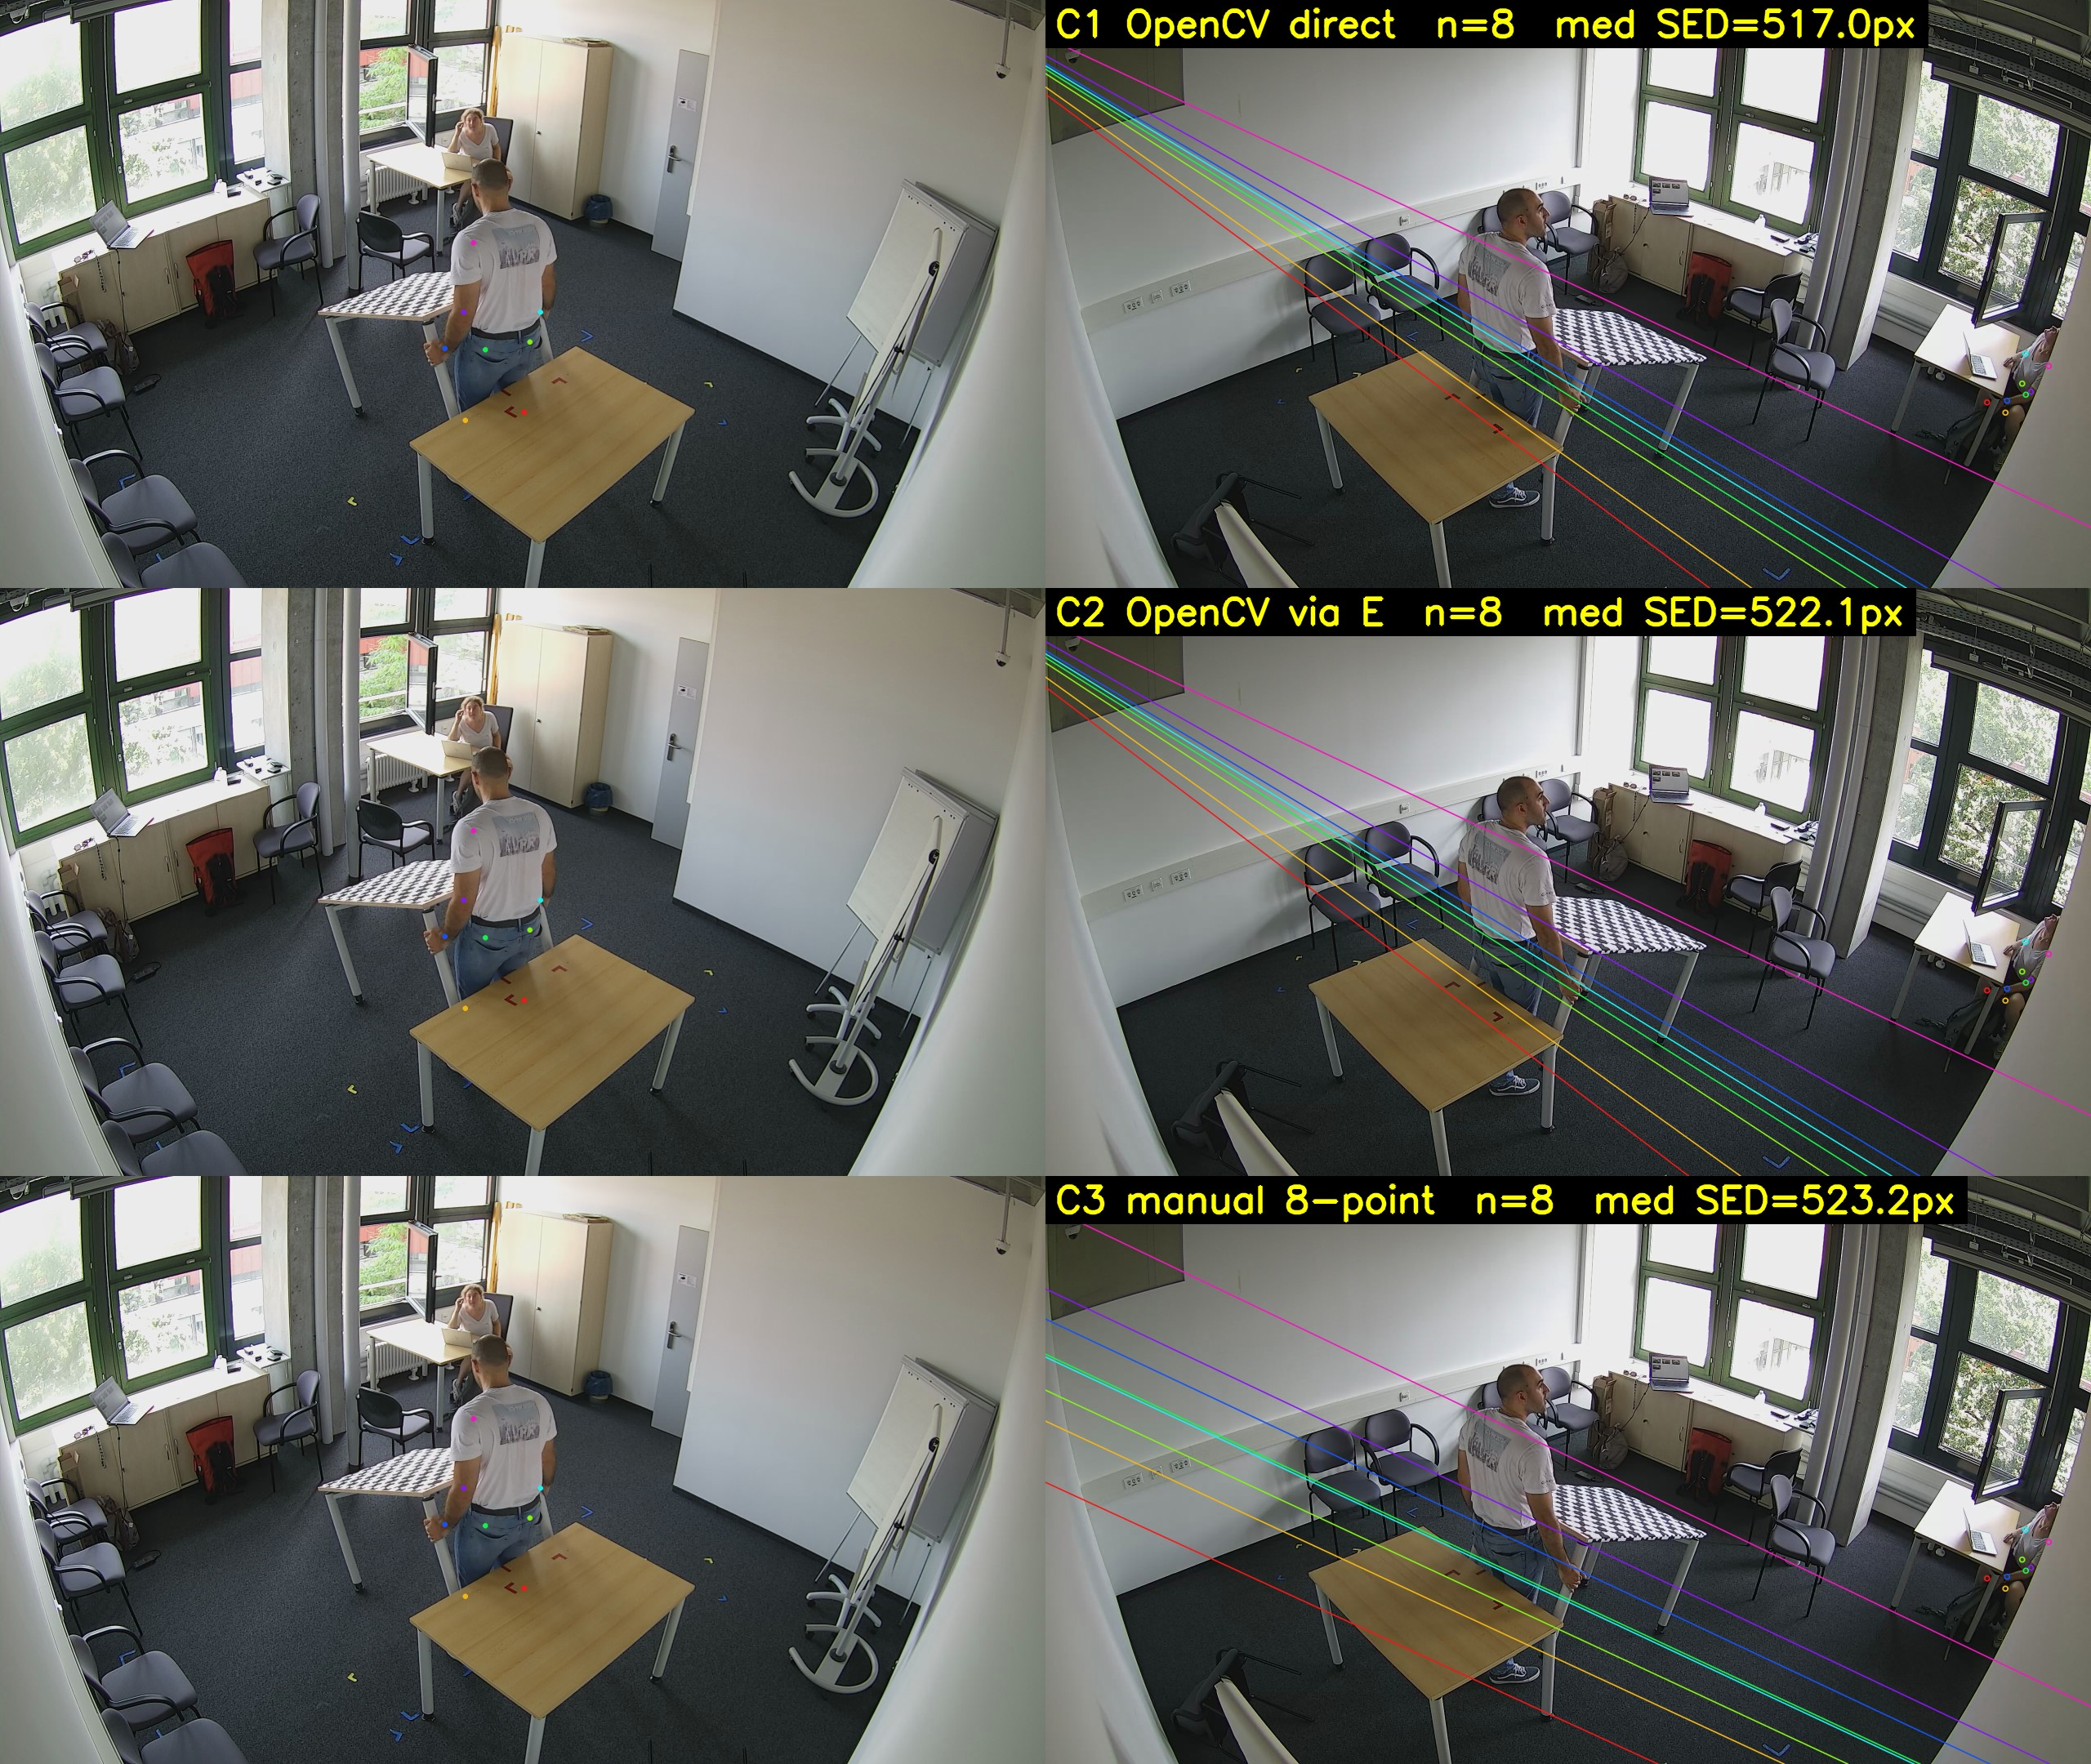
\includegraphics[width=\columnwidth]{figures/epipolar_f005968.jpg}
\vspace{-0.7cm}
\caption{Epipolar-line validation on frame $5968$ between \cam{0}
(left) and \cam{2} (right), using actor keypoint correspondences. The
lines no longer pass through their matched points for any of the
three methods (SED $\sim 500$~px on all three rows). This is not an
$F$ failure (the same $F$ matrices produced sub-pixel results on the
Puzzleboard test), but a correspondence and timing failure, discussed
in Section~\ref{sec:discussion}.}
\label{fig:epi-actor}
\end{figure}

\subsection{Discussion: which method works best}

For the Puzzleboard correspondences (the input that $F$ was fit on)
all three methods produce visually indistinguishable epipolar lines,
with median symmetric epipolar distance in the sub-pixel-to-few-pixels
range. Across our four tested frames, the via-$E$ estimator has the
lowest variance of error across frames because the essential-matrix
formulation makes use of the calibrated metric geometry; the direct
estimator is the most consistent baseline; the manual 8-point
sometimes wins on clean training frames (Figure~\ref{fig:epi-board})
and sometimes loses on near-degenerate ones, reflecting that our
manual implementation lacks the post-RANSAC nonlinear refinement
step.

On actor keypoint correspondences (Figure~\ref{fig:epi-actor}) all
three methods fail uniformly, with epipolar lines missing the
matched point by hundreds of pixels. The failure is the same across
methods, ruling out an $F$ defect, and points to a fundamental
problem upstream: the actor keypoint in camera A is matched to a
COCO-index sibling in camera B without any cross-camera identity
verification, so when the per-camera ``actor track'' filter picks a
different physical person in the two views (the moving actor in
\cam{0} but the seated bystander in \cam{2}, for example) the resulting
``correspondences'' are spurious. We return to this in the
discussion.

\section{Missing-Keypoint Recovery}
\label{sec:recovery}

\subsection{Method}

We treat one camera (\cam{0}) as the primary view and assume that for
some keypoint of interest its detection is missing in \cam{0} but
available in two supporting cameras, $a$ and $b$. For each
supporting view we compute the epipolar line that the support
observation projects into \cam{0}:
\begin{equation}
\ell_a \;=\; F_{0a}^{\top}\, x_a,
\qquad
\ell_b \;=\; F_{0b}^{\top}\, x_b,
\label{eq:epi-recovery}
\end{equation}
and recover the missing pixel as the intersection
$p = \ell_a \times \ell_b$ in homogeneous coordinates,
dehomogenising by dividing by the third component.

Because noisy detections and imperfect $F$ matrices mean the two
lines almost never intersect exactly at the true location, we
implement two safeguards. First, a near-parallel rejection rule:
if $|\sin \angle(\ell_a, \ell_b)| < 0.05$, the cross-product
intersection is numerically ill-conditioned and we fall back to the
\mbox{least-squares} solution. Second, when more than two supporting views
are available we always use the \mbox{least-squares} formulation: with
lines $\ell_i = (a_i, b_i, c_i)$ pre-normalised so $a_i^2 + b_i^2 =
1$, the point that minimises the sum of squared point-to-line
distances $\sum_i (a_i x + b_i y + c_i)^2$ is the closed-form
solution to a $2 \times 2$ linear system, which we obtain via
\texttt{numpy.linalg.lstsq}.

\subsection{Validation on Puzzleboard corners}

To separate the recovery algorithm from the cross-camera
correspondence problem, we first test on Puzzleboard corners, which
have unambiguous correspondences matched by piece id. For each test
frame we pick a corner that all four cameras see, recover the \cam{0}
pixel from the other cameras' observations, and compare against
\cam{0}'s actual detection.

\begin{table}[tbp]
\centering\small
\caption{Median recovery error on Puzzleboard corners with \cam{0} as
primary, under the canonical pipeline (undistorted-space $F$, sync-
corrected support frames). The 3-line LS reaches sub-pixel at a
static-board frame, validating that $F$ itself is geometrically
correct on its design distribution; the 2-line cross product is
fragile because intersection error scales as $1 / \sin \theta$ in
the angle between lines.}
\label{tab:recovery-board}
\begin{tabular}{|l|c|r|}
\hline
supports & method & median err \\
\hline
\cam{1}, \cam{2} & cross-product & 61.8 px \\
\cam{2}, \cam{3} & cross-product & 22.1 px \\
\cam{1}, \cam{2}, \cam{3} & LS over 3 lines & 0.66 px \\
\hline
\end{tabular}
\end{table}

The drop from tens of pixels to sub-pixel when switching from two to
three supports is not because the third $F$ is better individually;
it is because the cross-product intersection of two lines is
fragile when one of the lines has even a few pixels of noise. A
third line votes against any single-line outlier and the least-
squares solution averages across all three.

\subsection{Validation on actor keypoints}

The same method applied to actor keypoint correspondences gives a
median recovery error of 155~px on \cam{0} using \cam{1}+\cam{2}+\cam{3} as
supports under the original raw-pixel pipeline with constant
zero-offset synchronisation. This is two orders of magnitude worse
than the board-corner recovery on the same $F$, so the bottleneck is
not the recovery algorithm itself. We identify three independent
contributors, each measurable in isolation and each reducible by a
separate fix; together they account for the majority of the gap
between board and actor recovery.

\paragraph{Distortion absorbed into $F$.} The original pipeline fits
$F$ on raw distorted pixels and applies it to raw distorted query
points. The Brown--Conrady model produces median pixel shifts of
about 30~px at peripheral image positions, and an $F$ fit on raw
correspondences encodes a compromise that averages an
position-dependent distortion pattern across the harvest. At the
calibration moments (board near the image centre) this is
invisible; at peripheral test positions the bias surfaces as
additional epipolar-line error. Undistorting both sides before the
linear fit, doing the LS intersection in undistorted pixel space,
and re-distorting the recovered point back to raw pixel coordinates
for visualisation cuts the board-recovery error at a moving frame
from 190~px to 65~px and is itself sub-pixel on static frames.

\paragraph{Inter-camera temporal drift.} The four cameras' clocks
tick at different rates (Section~\ref{sec:sync}). Pairing
\cam{0} frame $N$ with cam $c$ frame $N$ at harvest time embeds the
drift into the correspondence set, and the 8-point algorithm
finds the best compromise $F$ given the slightly-mismatched pairs.
Pairing \cam{0} frame $N$ with cam $c$ frame
$\textnormal{round}(\alpha_c + \beta_c\,N)$ at harvest time gives
the algorithm physically-simultaneous correspondences and tightens
the resulting $F$ accordingly. The \cam{0}--\cam{3} inlier SED falls
from 10.68~px in the original harvest to 1.45~px in the
synced-and-undistorted refit (Table~\ref{tab:F-results}), with
\cam{3}'s drift accounting for most of the difference.

\paragraph{Rolling-shutter shear during motion.} The cameras are
CMOS sensors with row-by-row exposure: the top row of each frame is
captured several milliseconds before the bottom. When the subject
is static, every row sees the subject at the same physical position
and the shear is invisible. When the subject is moving, the
captured image is sheared in the temporal-spatial sense, and no $F$
fit under the global-shutter assumption can satisfy the epipolar
constraint exactly. We confirm this directly: at moving-board
frames the per-corner SED correlates strongly with image y-position
($r = -0.87$ at frame 1200, $r = -0.71$ at frame 4450), while at
static-board frames the correlation is negligible ($r = -0.11$ at
frame 6450). The signature points unambiguously at rolling shutter,
which is a property of the hardware rather than the model.

After applying the undistort-first refit and the event-anchored sync
end-to-end, the best actor recovery configuration we obtain is
\cam{1}+\cam{2} with two-support cross-product intersection in
undistorted space, re-distorted to raw pixels for the error
metric: median 68.21~px across 117 keypoint recoveries on 12
evenly-spaced frames (Table~\ref{tab:e1-progression}). This is a
56\% reduction from the 155~px baseline. The residual is
attributable to the third effect above plus cross-view
anatomical drift in YOLO keypoint positions (the same COCO label
identifies slightly different anatomical points across views with
markedly different angles), both of which are out of scope for
this implementation.

\begin{table}[tbp]
\centering\small
\caption{End-to-end progression of actor-keypoint recovery error,
median over 12 evenly-spaced test frames with \cam{0} as primary. Each
row adds one correction to the row above; the supports column lists
the configuration that minimises median error under that pipeline.}
\label{tab:e1-progression}
\begin{tabular}{|l|l|r|}
\hline
pipeline & supports & median \\
\hline
baseline\textsuperscript{*}    & \cam{1}+2+3 & 155 \\
+ undistort                    & \cam{1}+2+3 & 127 \\
+ event sync                   & \cam{1}+2+3 & 79 \\
+ 2-support                    & \cam{1}+2   & 68 \\
\hline
\end{tabular}\\[2pt]
{\footnotesize \textsuperscript{*}raw-pixel $F$, raw-pixel inputs, $\tau = 0$. Errors in pixels.}
\end{table}

\begin{figure}[tbp]
\centering
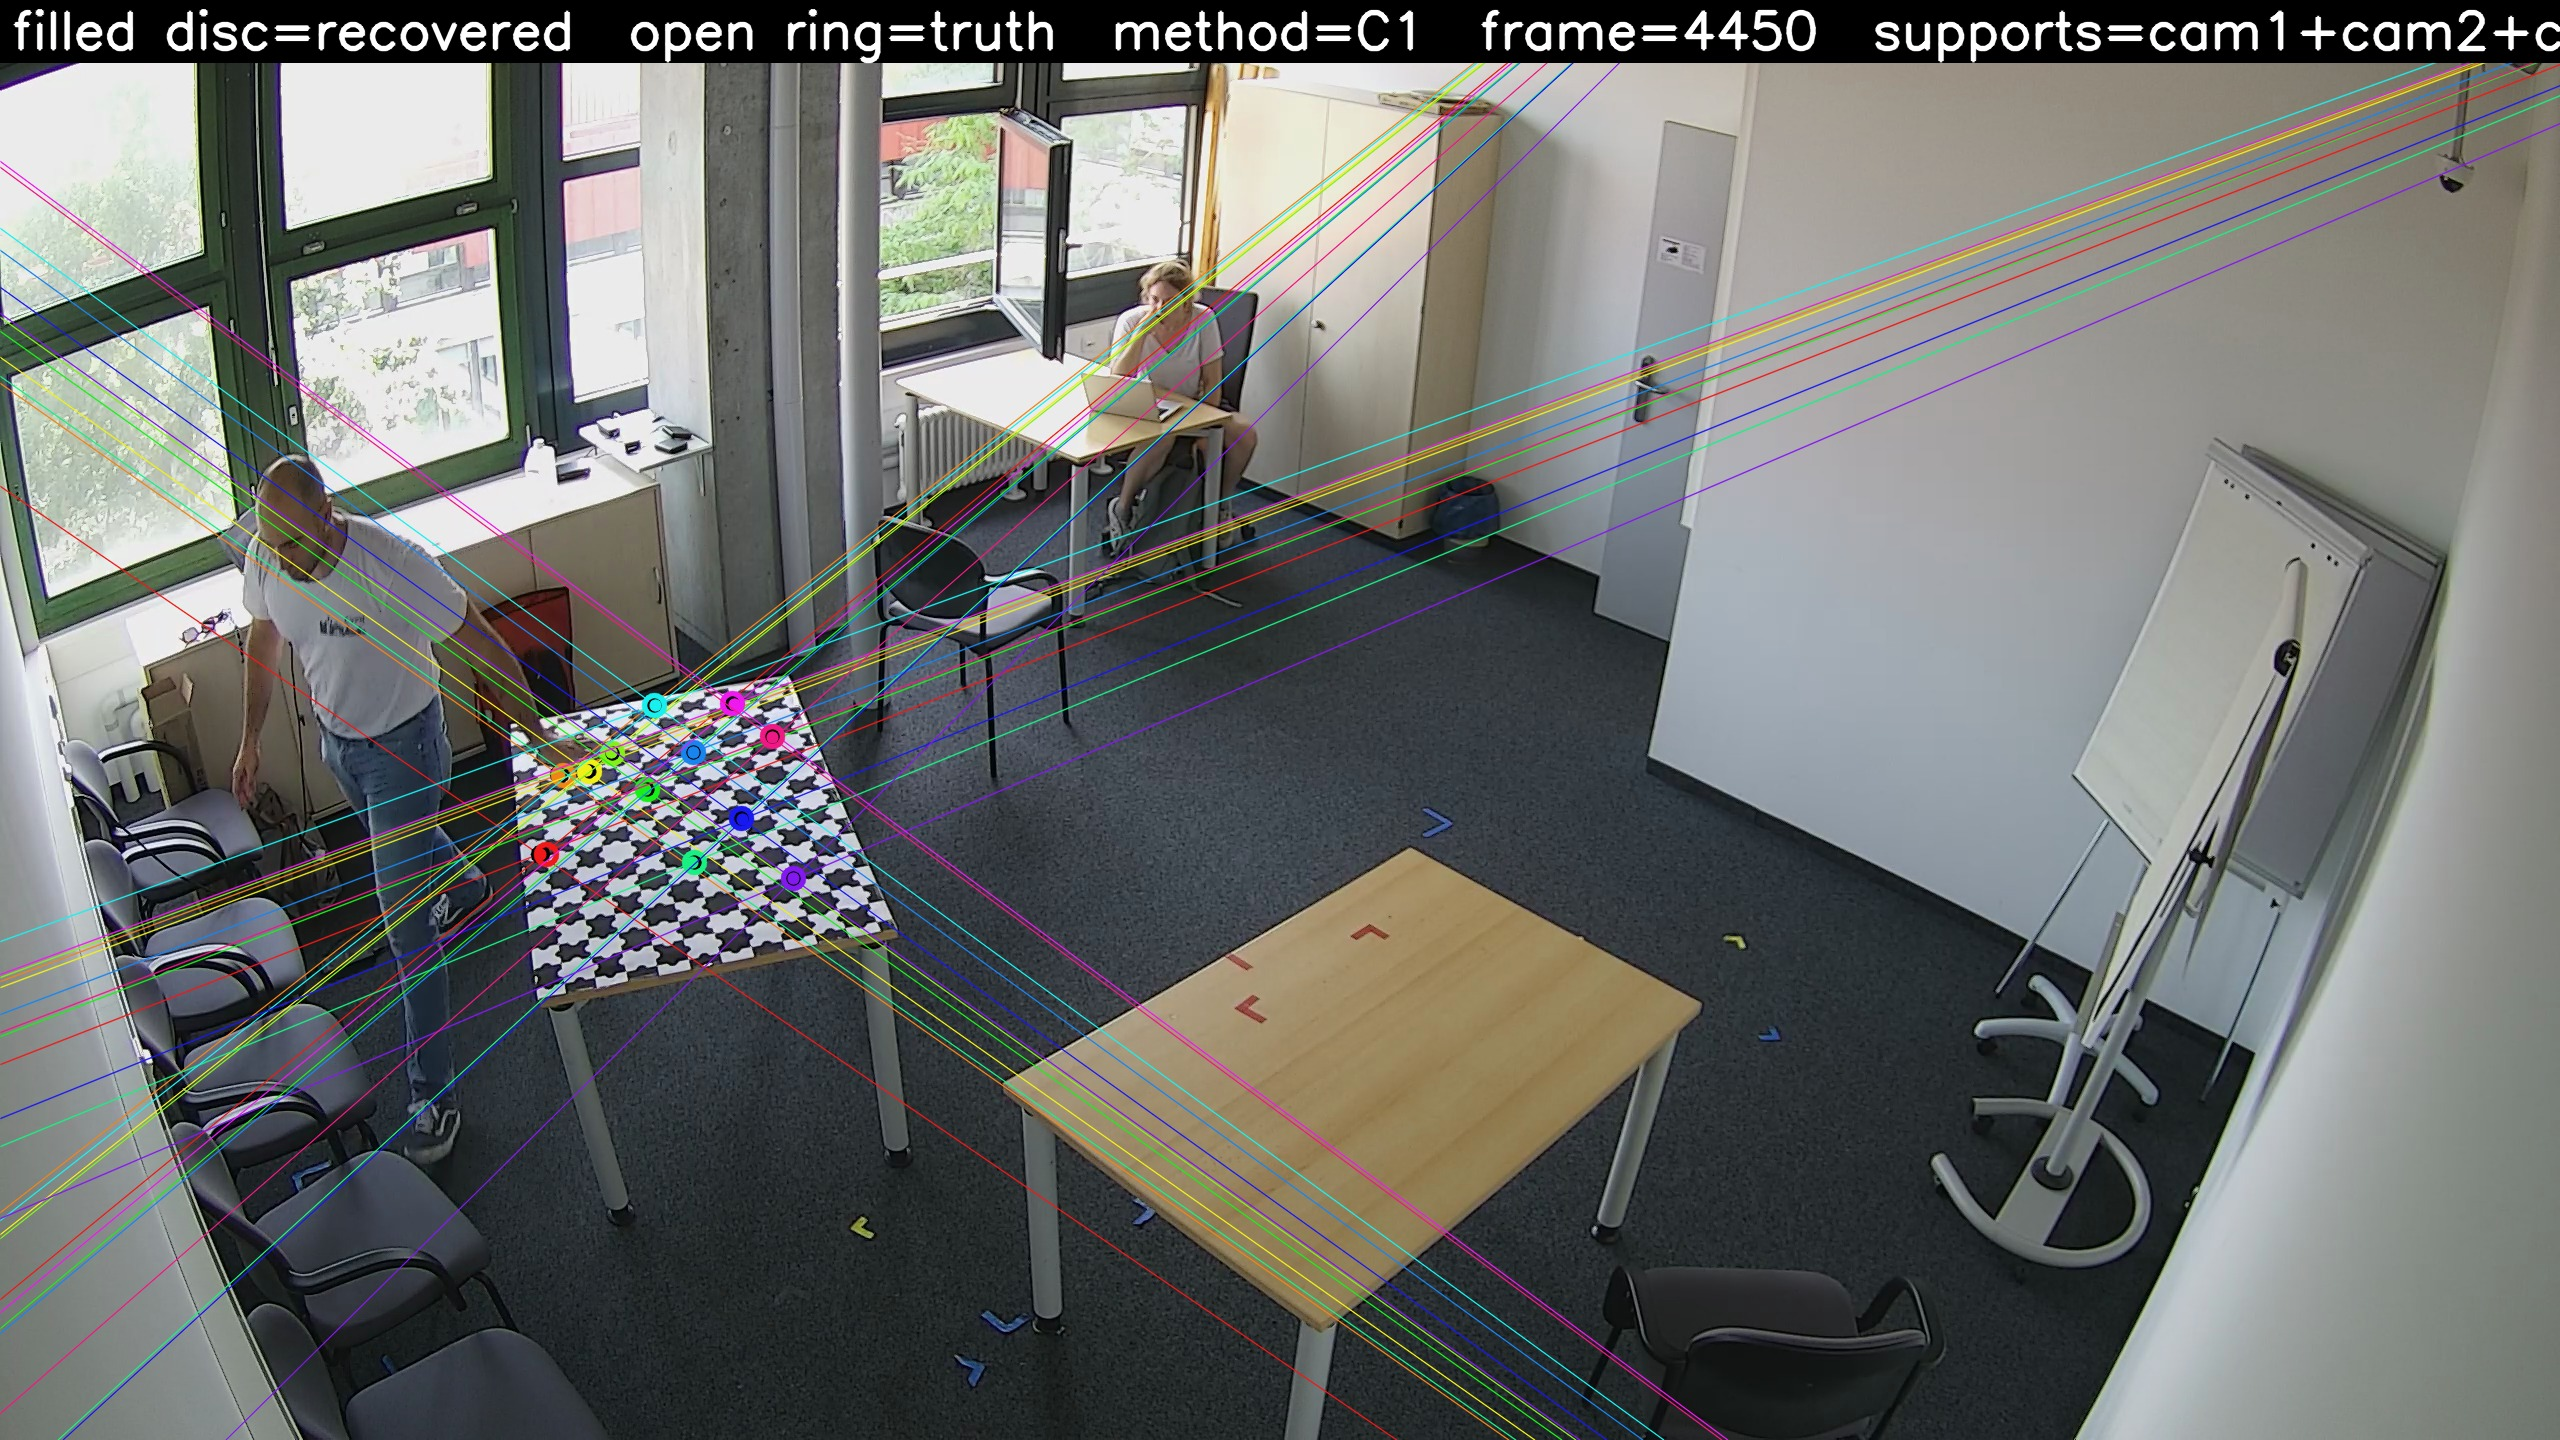
\includegraphics[width=\columnwidth]{figures/recovery_board.jpg}
\vspace{-0.7cm}
\caption{Missing-keypoint recovery on Puzzleboard corners, \cam{0} as
primary with \cam{1}+\cam{2}+\cam{3} as supports. For each tested corner we
draw the three epipolar lines from the supporting cameras (thin
coloured lines), the recovered location (filled disc), and the
ground-truth location of that corner in \cam{0} (open ring of the same
colour). The filled discs and the rings sit at essentially the same
pixels.}
\label{fig:rec-board}
\end{figure}

\subsection{What happens when the lines do not intersect cleanly}

In the two-line cross-product formulation, ``not cleanly'' covers two
regimes. If the lines are far from parallel but each carries
moderate noise (a few pixels per line), the recovered point is
typically within a few tens of pixels of the truth, with the error
scaled by the inverse sine of the angle between the lines. If the
lines are near-parallel (very acute or obtuse intersection angle)
the recovered point becomes essentially unbounded; this is the case
caught by our \texttt{parallel\_threshold} check, where we refuse
the cross-product answer and fall back to least squares.

In the \mbox{least-squares} formulation, ``not cleanly'' is handled
gracefully and the recovered point is the one that minimises the
total geometric error to all lines simultaneously. The cost is that
a single bad line (whether from a bad detection or a noisy $F$)
still biases the solution; a more sophisticated implementation could
add a RANSAC layer over the lines themselves to discard one-off
outliers, but our experiments with three supports show that the
plain LS is already enough in practice when the supporting $F$
matrices are of comparable quality.

\section{Discussion and Limitations}
\label{sec:discussion}

The most consequential single finding is the calibration edge-corner
ablation (Section~\ref{sec:edge-ablation}): filtering the detector
output by row/column extremum improved monocular RMS by 60--70\% on
all four cameras. Respecting the planarity assumption matters more
than maximising the point count, and a planar-target calibration
above 1.5~px RMS on a modern camera should treat a curl-affected
outer ring as the first suspect.

Two corrections at harvest time shape every downstream number. The
first is undistortion: fitting $F$ on raw distorted pixels lets
the rank-2 matrix absorb a position-dependent error pattern that
masquerades as geometry, and recovery on out-of-distribution test
positions surfaces it as additional epipolar-line error. Undistorting
both sides via the per-camera $(K, D)$ before the linear fit, doing
the LS intersection in undistorted pixel space, and re-distorting
the recovered point only for display restores clean pinhole
geometry. The second is event-anchored synchronisation: the NCC
estimator we initially used returns $\tau = 0$ at integer
resolution but cannot represent the linear drift driven by 1\% FPS
mismatch across the cameras. A two-event affine fit produces an
$(\alpha, \beta)$ pair per support camera that captures both the
start-time offset and the rate ratio exactly; \cam{3}'s drift of 142
frames over the recording is the most consequential and the most
invisible to NCC.

The residual on actor recovery after both corrections is dominated
by two effects that are visible in the \mbox{diagnostics} but out of scope
for this implementation. The first is cross-view anatomical drift
in YOLO keypoint positions: the same COCO label identifies slightly
different anatomical points across views with markedly different
camera angles, and the resulting cross-camera correspondence noise
amplifies through the LS intersection. The second is rolling-shutter
shear during subject motion, whose strong y-position correlation in
the SED data we report in Section~\ref{sec:recovery}. The first is
addressable by a higher-capacity keypoint detector or by per-view
re-identification at correspondence time; the second is a hardware
limit and would require either global-shutter cameras or an explicit
rolling-shutter model embedded in the epipolar geometry.

A smaller methodological note: our manual $F$ estimator omits the
post-RANSAC Levenberg--Marquardt step that
\texttt{cv2.findFundamentalMat} performs. The linear eight-point
step itself matches \texttt{FM\_8POINT} to $10^{-10}$; the gap to
\texttt{FM\_RANSAC} on held-out points is entirely in this
refinement. Adding LM with a rank-2-preserving parameterisation of
$F$ would close it.

\section{Conclusion}
\label{sec:conclusion}

We implemented an end-to-end multi-view human-tracking pipeline
covering all assignment tasks: sub-pixel calibration on all four
cameras (after dropping the curl-affected outer ring of Puzzleboard
corners), an event-anchored affine synchronisation model fit from
two manually-identified board-impact events,
$\geq 95\%$ YOLO-pose detection coverage, an actor-only best-view
composite video, three independently-estimated fundamental matrices
agreeing to within 1\% Frobenius distance, and a missing-keypoint
recovery method reaching 0.66~px median error on Puzzleboard corners
with three supporting views.

On actor keypoints the recovery median is 68.21~px across 117
recoveries in 12 evenly-spaced test frames, a 56\% reduction from
the 155~px baseline obtained with raw-pixel $F$, raw-pixel inputs,
and a constant-zero sync model. The forensic stage of the report
attributes the remaining error to two effects we measure but do not
fully resolve: cross-view anatomical drift in YOLO keypoint
positions, and rolling-shutter shear during subject motion.

Two practical lessons stand out. First, respecting the assumptions
of the underlying algorithm (Zhang's planarity for calibration, the
pinhole projection for $F$, the global-shutter assumption embedded
in both) is worth more than the easy levers of more frames or more
correspondences. Second, redundancy across supporting cameras under
LS intersection robustifies recovery on clean correspondences, but
at moving-actor frames a single mis-aligned support can amplify the
LS residual rather than dampen it: the wider-baseline two-camera
configuration with a clean $F$ outperforms the three-camera LS in
our final result for this reason.

\begin{thebibliography}{9}

\bibitem{zhang2000}
Z.~Zhang.
\newblock A Flexible New Technique for Camera Calibration.
\newblock {\em IEEE Transactions on Pattern Analysis and Machine
Intelligence}, 22(11):1330--1334, 2000.

\bibitem{brown1971}
D.~C.~Brown.
\newblock Close-Range Camera Calibration.
\newblock {\em Photogrammetric Engineering}, 37(8):855--866, 1971.

\bibitem{hartley1997}
R.~Hartley.
\newblock In Defense of the Eight-Point Algorithm.
\newblock {\em IEEE Transactions on Pattern Analysis and Machine
Intelligence}, 19(6):580--593, 1997.

\bibitem{hartley2003}
R.~Hartley and A.~Zisserman.
\newblock {\em Multiple View Geometry in Computer Vision}.
\newblock Cambridge University Press, 2nd edition, 2003.

\end{thebibliography}

\end{document}
